\documentclass[12pt]{article}

% ============================================================
% Preamble
% ============================================================
\usepackage[margin=1in]{geometry}
\usepackage[utf8]{inputenc}
\usepackage[T1]{fontenc}
\usepackage{amsmath,amssymb}
\usepackage{graphicx}
\usepackage{booktabs}
\usepackage{longtable}
\usepackage{array}
\usepackage{caption}
\usepackage{subcaption}
\usepackage{rotating}      % sideways tables/landscape appendix tables
\usepackage{pdflscape}
\usepackage{chngcntr}      % \counterwithin, for appendix table/figure numbering (A1, B1, ...)
\usepackage[section]{placeins} % keeps floats from drifting past the section that introduces them
\usepackage{setspace}
\usepackage{titlesec}
\usepackage{natbib}
\usepackage{hyperref}
\hypersetup{colorlinks=true, linkcolor=blue, citecolor=blue, urlcolor=blue}
\usepackage[skip=6pt, indent=0pt]{parskip}

% Extra breathing room throughout: line spacing, paragraph spacing,
% table row height, and spacing around section headings.
\setstretch{1.2}
\setlength{\parskip}{6pt plus 1pt minus 1pt}
\renewcommand{\arraystretch}{1.25}
\setlength{\tabcolsep}{6pt}
\titlespacing*{\section}{0pt}{28pt plus 4pt minus 2pt}{14pt plus 2pt}
\titlespacing*{\subsection}{0pt}{20pt plus 3pt minus 2pt}{10pt plus 2pt}
\bibliographystyle{apalike}

\newcommand{\notes}[1]{\par\vspace{8pt}\footnotesize\noindent\textit{Notes:} #1\par\vspace{2pt}}
\newcommand{\source}[1]{\par\vspace{4pt}\footnotesize\noindent\textit{Source:} #1\par\vspace{2pt}}

\title{The Aftermath of Sovereign Spread Crises With and Without Default}
\author{}
\date{\today}

% ============================================================
\begin{document}
\maketitle

% ------------------------------------------------------------
\begin{abstract}
\noindent
Sovereign debt crises are not necessarily accompanied by default, as severe
episodes of market distress can also occur without missed payments or debt
restructuring. In this paper we examine the macroeconomic dynamics of
sovereign debt crises without default and compare them with crises with
default. Using the JP Morgan EMBIG spread for 52 countries from 1994
onward, we identify 40 spread crises without default and 21 spread crises
with default. Our augmented inverse probability weighted (AIPW) local
projection estimates show that GDP and domestic bank credit to the private
sector are largely unaffected during crises without default but contract
substantially during crises with default. Investment, however, declines by
a similar magnitude across both types of crises, with no robust difference
between them. Extending the analysis to domestic banks' exposure to the
sovereign, we find that, among debt crises without default, high exposure
is associated with a significantly better GDP outcome than low exposure.
However, among crises with default, the difference between countries with
high and low sovereign exposure does not appear to be statistically
significant for any outcome.
\end{abstract}

\newpage
\tableofcontents
\newpage

% ============================================================
\section{Introduction}
% ============================================================

Sovereign debt crises are recurring events in emerging markets and, over
recent decades, have frequently been resolved through debt restructuring.
The literature on sovereign debt crises has consequently devoted
considerable attention to measuring the costs of sovereign default. As
discussed by Ams et al.\ (2019), researchers and rating agencies typically
identify a sovereign default as involving either (i) missed payments or a
legal default, or (ii) a debt restructuring on terms less favourable than
the original terms, resulting in creditor losses (``haircuts'') and/or
coercion imposed by the sovereign. However, not all sovereign debt crises
fall within this definition. During the eurozone crisis, bondholders
continued to receive payments in full and on time. In a similar vein,
several prominent emerging market crises, such as in Mexico (1994/95),
Thailand (1997/98), Brazil (1999 and 2002), Turkey (2001), or Russia (2015)
did not result in a default or restructuring of external debt (Mitchener
and Trebesch, 2021).

Pescatori and Sy (2007) argue that a default-only definition of debt
crises becomes problematic once sovereign bond markets emerge in
developing economies. They demonstrate that default episodes have grown
increasingly unreliable as a signal of debt distress and call instead for
a broader measure grounded in bond market turbulence. On this basis, they
extended the definition of debt crises to episodes in which yield spreads
exceed 1000 basis points, a threshold they describe as a ``psychological
barrier'' for market participants. A similar approach is adopted by
Broner, Lorenzoni, and Schmukler (2013) and Aguiar et al.\ (2016), who
characterize debt crises through sharp quarter-on-quarter increases in
bond yields, a phenomenon later termed ``spread crises'' or ``spread
spikes'' by Krishnamurthy and Muir (2017). Mitchener and Trebesch (2021)
introduce the term ``sovereign debt crisis without a default'' to describe
episodes marked by elevated sovereign bond yields and debt rollover
difficulties in the absence of missed payments or formal default. Their
evidence indicates that such episodes are not a novel phenomenon, though
their frequency has risen markedly since the 1990s.

This paper evaluates the macroeconomic cost of sovereign debt crises
without default and asks how that cost compares to episodes that do end in
default. The analysis draws on the JP Morgan EMBIG spread database to
identify episodes of sovereign spread distress. Following the combined
approach of Pescatori and Sy (2007), Aguiar et al.\ (2016), and
Krishnamurthy and Muir (2017), a spread crisis episode is defined as
beginning in the first year in which a country enters sovereign spread
distress following at least one tranquil year. Following the logic of
Detragiache and Spilimbergo (2001), consecutive distress years are treated
as part of the same episode, and a one-year interruption rule applies: a
single non-crisis year surrounded by crisis years does not terminate the
episode, which is instead treated as continuous, and an episode is
considered concluded only once two consecutive non-crisis years follow.
Each identified crisis episode is then cross-referenced with the Asonuma
and Trebesch (2016) sovereign restructuring database, extended to
incorporate post-2020 restructuring events. Episodes concurrent with a
formal sovereign restructuring are classified as default-linked; the
remainder are classified as debt crises without default. This approach
identifies 61 spread crises, of which 21 (34 percent) coincide with an
outright default and 40 do not.

We apply local projection with the Augmented Inverse Probability Weighted
(AIPW) method of Jord\`a and Taylor (2016) to attenuate selection bias and
estimate the dynamic responses of GDP, investment, bank credit to the
private sector, bank claims on government, FDI, and real lending rates for
each type of spread crisis. We extend our analysis by applying the AIPW
estimation on two samples differentiated by whether the sovereign-bank
nexus in the year prior to the start of the spread crisis is higher than
the median across all spread crisis episodes. With this approach, proposed
by Auerbach and Gorodnichenko (2016) and Jord\'a and Taylor (2016), we
quantify not only how our macroeconomic aggregates respond to a sovereign
spread crisis, but also how the pre-crisis exposure of the domestic
banking system to the sovereign shapes the amplification of that response.

Our results show four main findings. First, GDP and bank credit to the
private sector exhibit the clearest and most persistent differences
between crises with and without default. Following crises without
default, GDP declines modestly, by around 1--2 percentage points over the
first two years, before returning towards its pre-crisis path. By
contrast, GDP falls by 6--9 percentage points following crises with
default, with the decline remaining significant five years after the
crisis onset. Bank credit displays a similar, but more delayed, contrast:
it turns significantly positive by the fifth year following crises
without default, reaching nearly 7 percentage points above its pre-crisis
path, while falling to almost 40 percentage points below its pre-crisis
path following crises with default. Second, this distinction is less
apparent for investment, FDI, and real lending rates. Investment declines
by a broadly similar magnitude following both types of crises, while the
responses of FDI and real lending rates do not differ significantly
between the two types of crises at any horizon. Third, claims on
government increase sharply in the crisis year following crises with
default, by around 7 percentage points, while remaining broadly unchanged
following crises without default. Finally, the pre-crisis sovereign-bank
nexus does not systematically amplify the output costs of crises with
default, although point estimates tend to be more negative when sovereign
exposure is high. For crises without default, by contrast, higher
pre-crisis sovereign exposure is associated with a significantly better
GDP response on impact.

\paragraph{Related literature.} This paper relates to three strands of
the literature on sovereign debt.

The first is the literature on debt crises without default. Pescatori and
Sy (2007), Aguiar et al.\ (2016), and Krishnamurthy and Muir (2017) define
these episodes through bond-market distress rather than through a missed
payment. Bocola (2016) shows theoretically that expectations of a future
default can tighten bank lending and depress output even absent an actual
default. Mitchener and Trebesch (2021) document that such episodes have
become increasingly common since the 1990s. None of this work offers
systematic cross-country evidence on the aggregate output effects of
these crises, which is the gap we fill.

Second, this paper relates to the literature on the output cost of
sovereign default. Borensztein and Panizza (2009), Furceri and Zdzienicka
(2012), Trebesch and Zabel (2017), and Kuvshinov and Zimmermann (2019)
estimate this cost at 1 to 4 percentage points of GDP per capita growth,
typically without benchmarking it against a comparable sample of equally
severe episodes that did not end in default. Levy Yeyati and Panizza
(2011) show that most output contraction occurs before the default
itself, a finding that motivates our design of comparing default-linked
and non-default crises within the same estimation framework rather than
comparing default to tranquil years alone. We build on this work by
estimating both crisis types jointly and showing that GDP and bank credit
to the private sector fall considerably more, and for longer, in
default-linked crises, while investment and the response of FDI and real
lending rates do not differ significantly across the two.

Third, this paper relates to the sovereign-bank nexus literature, which
is built largely on euro-area or single-country microdata. Gennaioli,
Martin, and Rossi (2014) and Acharya, Eisert, Eufinger, and Hirsch (2018)
emphasize bank holdings of sovereign debt as a channel through which
sovereign distress transmits to credit and output, and Bocola (2016)
models the anticipatory version of this channel. Asonuma, Chamon, Erce,
and Sasahara (2024) measure exposure using a credit-to-GDP ratio, whereas
we use the pre-crisis share of bank assets held as claims on government.
This literature, together with Acharya and Steffen (2015) and Acharya,
Drechsler, and Schnabl (2014) on banks' tendency to absorb rather than
shed sovereign risk during distress, is consistent with our finding that
claims on government rise sharply in the crisis year following
default-linked crises but not following crises without default. We
extend this literature by comparing high- and low-exposure countries
across both crisis types rather than within a single one, and find a
significantly better GDP response to high exposure in crises without
default, with no significant difference in crises with default.

% ============================================================
\section{Data Description and Classification of Spread Crises}
% ============================================================

Throughout the paper, we focus on episodes of sovereign spread distress
identified from JP Morgan EMBIG spread data, classified as default-linked
or as debt crises without default based on whether the episode coincided
with a private external debt restructuring. Our sample covers the period
1993--2025 and includes the full panel of countries covered by EMBIG
spread data. We retain these countries because our propensity model is
estimated without country fixed effects, given the relatively small
number of default-linked episodes in our sample; a pooled propensity
model uses every tranquil and onset year across the panel as informative
observations, so a country with no default-linked episode of its own
still contributes to identifying the propensity score. Our sample has 52
countries, which are listed in Table~\ref{tab:A1} of Appendix~A.

We date the start and continuation of each spread crisis episode
following the interruption rule: a single tranquil year surrounded by
distress years does not split one episode into two, and an episode is
considered concluded only once two consecutive tranquil years follow.
This rule is applied directly to the annual spread data and determines,
from the data itself, whether two nearby periods of distress constitute
one episode or two, without requiring a separately imposed window or rule
for overlapping events.

Each identified episode is classified as default-linked or as a debt
crisis without default by cross-referencing it against the Asonuma and
Trebesch (2016) sovereign restructuring database, extended to incorporate
post-2020 restructuring events. An episode is classified as default-linked
if it coincides with, or is followed during the episode by, a formal
sovereign debt restructuring. All other episodes are classified as debt
crises without default. We use this binary classification because our
object of interest is whether a period of sovereign market stress
culminates in default at all, rather than the terms on which any
subsequent default is resolved. We identify 61 spread crisis episodes, of
which 21 (34 percent) are default-linked and 40 are debt crises without
default. Table~\ref{tab:A2} in Appendix~A presents the list of spread
crisis episodes.

We code each episode as a single onset-year event: the treatment dummy
for a given episode is set to unity in the year the episode begins and
zero in all other years, including years during which the episode
continues. This lets each episode enter the estimating equation as one
treated observation, consistent with the annual local-projection
framework used throughout the paper.

For macroeconomic variables, we use data at an annual frequency in order
to secure the widest possible country coverage. The data sources include
the following: IMF World Economic Outlook for GDP, prices, government
expenditure, and other national accounts variables; World Bank World
Development Indicators (WDI) for bank credit to the private sector, trade
openness, and related indicators; IMF International Financial Statistics
for the sovereign-bank nexus variables (bank claims on government and on
the private sector, relative to total bank assets); World Bank
International Debt Statistics for external debt composition and
debt-service indicators; FRED for the US federal funds rate; and Laeven
and Valencia (2013, 2020) for the banking crisis dummy. Distance weights
used in the construction of the contagion predictor are built from
great-circle distances between capital cities, based on the CEPII
geographic database. Sources and summary statistics for our variables are
reported in Table~\ref{tab:A3} and Table~\ref{tab:A4} of Appendix~A.

% ============================================================
\section{Stylized Facts: Ordinary Least Squares Local Projection Estimation}
% ============================================================

We start by presenting stylized facts based on both sample means and
Ordinary Least Squares (OLS) estimation. Figure~\ref{fig:1} reports the
average cumulative percentage changes relative to the pre-crisis level
($t=0$, one year before the onset of the spread crisis) for GDP,
investment, bank credit, claims on government, FDI, and the real lending
interest rate. The series are adjusted for differences in country means,
corresponding to country-specific linear trends in levels, computed over
the estimation sample. Spread crises begin at $t=1$. Figure~B1 in
Appendix~B reports the dynamics of these macroeconomic variables during
the three years preceding the crisis. GDP and investment exhibit larger
declines in the years leading up to default-linked spread crises,
highlighting the importance of controlling for initial macroeconomic
conditions in both the first and second stages of the estimation.
Figures~B2 and B3 in Appendix~B replicate Figure~\ref{fig:1} and Figure~B1
using sample medians rather than means and yield similar patterns.

\begin{figure}[htbp]
\centering
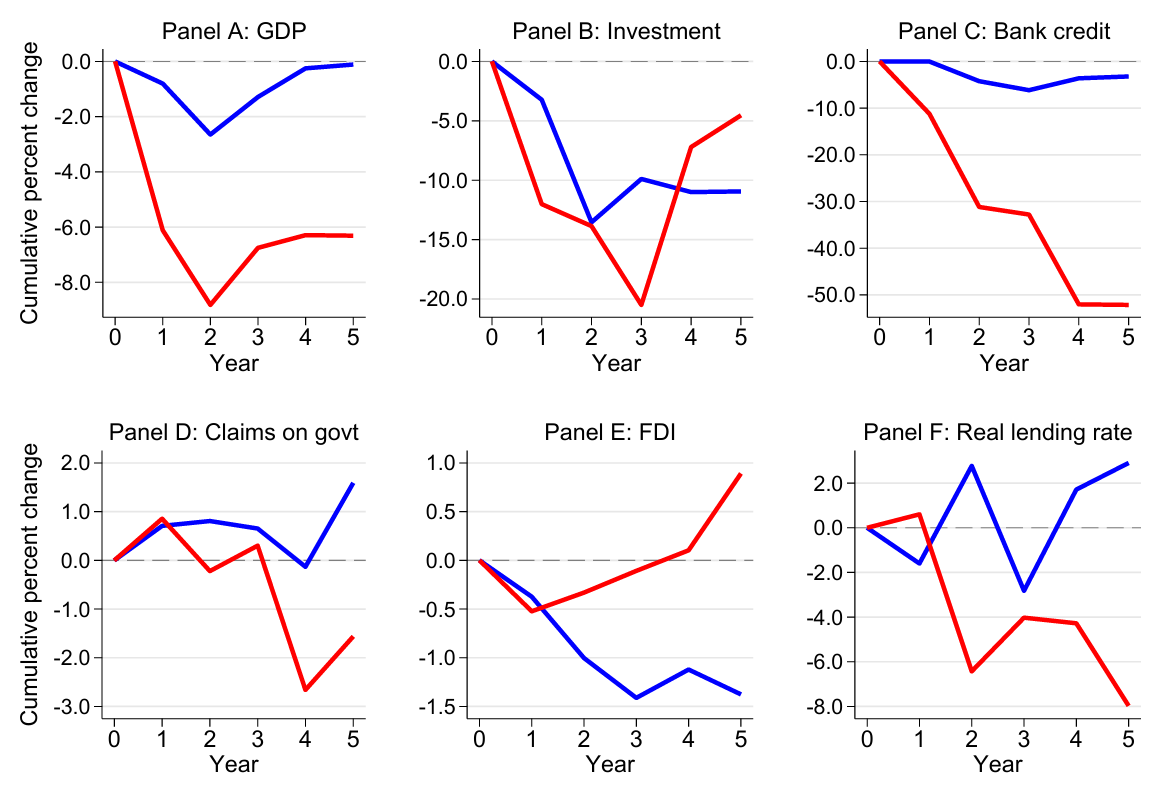
\includegraphics[width=0.95\textwidth]{figures/fig1_mean_dynamics.png}
\caption{Key variables around spread crisis onsets, mean.}
\label{fig:1}
\notes{GDP, investment, and bank credit series are the averages of
demeaned cumulative percentage changes from the level in the year before
the start of a spread crisis ($t=0$). Claims on government, FDI, and the
real lending interest rate series are the averages of demeaned cumulative
changes from the level in the year before the start of a spread crisis
($t=0$).}
\end{figure}

Both GDP and bank credit experience severe losses following a
default-linked spread crisis (red lines in Panels A and C), while the
effect of a non-default spread crisis tends to remain mild. Negative
values indicate the percentage deviation of GDP or bank credit from their
country-specific pre-crisis dynamics. These deviations remain sizeable for
several years following the crisis. Investment declines in both groups,
although the timing and magnitude of the contraction differ. In
default-linked crises, the trough occurs later and is deeper, reaching its
lowest point in year 3, compared with year 2 for non-default crises. By
year 5, however, the pattern reverses: investment begins to recover in
default-linked crises, while it remains depressed following non-default
crises.

Claims on government (Panel D) increase in both groups following the
onset of the crisis, suggesting that countries tend to rely more heavily
on domestic financial markets to meet their financing needs. This
increase is subsequently reversed, with claims on government declining
after year 3. FDI also declines in both groups in the years immediately
following the onset. However, the subsequent dynamics differ markedly:
FDI rebounds following default-linked crises, becoming positive by year 5
(Panel E, red line), whereas it remains below its pre-crisis dynamics
throughout the horizon following non-default crises (Panel E, blue line).

Real lending interest rates (Panel F) remain broadly stable in the
short-term following default-linked crises but decline sharply over the
medium term. This decline appears to be driven primarily by a surge in
inflation rather than by nominal lending rates, which have turned
negative by that stage (red line in Panel F). This pattern is largely
absent following non-default crises, for which neither inflation nor
nominal lending rates exhibit a clear trend over the horizon (blue line in
Panel F). Figure~B4 in Appendix~B reports the average cumulative changes
in inflation, measured by the GDP deflator, and in nominal lending
interest rates separately. It shows that the dynamics of real lending
interest rates in the default-linked group closely track those of
inflation rather than those of nominal lending rates.

We employ the local projection approach of Jord\`a (2005) to estimate the
cumulative effect of a spread crisis over a horizon $h$. We estimate two
separate regressions for non-default and default-linked spread crises.
Control variables are defined as those that influence the evolution of a
country's spread and are, in turn, influenced by the occurrence of a
spread crisis. The baseline local projection specification follows the
set of lagged controls in Asonuma et al.'s (2024) and includes: (i) GDP
growth, (ii) government expenditure-to-GDP ratio, (iii) trade openness
(exports + imports / GDP ratio), (iv) banking crisis dummy, (v) bank
credit-to-GDP ratio, (vi) inflation, (vii) nominal exchange rate
depreciation, and (viii) debt-to-GDP ratio. Table~D1 in Appendix~D shows
differences in macroeconomic variables for both treatment and control
groups in the year of the start of the spread crisis onset and one year
before, and results justify our selection of controls.

Our baseline model specification follows Jord\`a and Taylor (2016) and
this project's own onset-tier design. We estimate two outcome forms, the
cumulative log change for GDP, investment, bank credit, and the real
lending interest rate, and the cumulative level (percentage-point) change
for claims on government, FDI, and the two sovereign-bank exposure
shares, from the pre-crisis year (year $t-1$) to year $t+h$, separately
for each crisis type $S \in \{\text{non-default}, \text{default-linked}\}$,
as follows:

\begin{equation}
\label{eq:1}
y_{i,t+h} - y_{i,t-1} = \alpha_i^{S,h} + \beta^{S,h}\, D_{i,t}^{S}
  + \Gamma^{S,h\prime} X_{i,t-1} + \varepsilon_{i,t+h}^{S}
  \qquad \text{(untreated / treated combined OLS form)}
\end{equation}

\begin{equation}
\label{eq:2}
E\!\left[\, y_{i,t+h} - y_{i,t-1} \;\middle|\; D_{i,t}^{S}=d,\, X_{i,t-1} \,\right]
  = m_d^{S,h}(X_{i,t-1}), \qquad d \in \{0,1\}
\end{equation}

\noindent where, for each horizon $h=1,2,\dots,5$ and each type of spread
crisis $S=\{\text{non-default}, \text{default-linked}\}$, $\alpha_i^{S,h}$
denotes country fixed effects, $D_{i,t}^S$ indicates the dummy variable
taking unity when a spread crisis of type $S$ occurs in year $t$, and
$\beta^{S,h}$ is its coefficient. The vector of control variables is
denoted by $X_{i,t-1}$, with coefficients $\Gamma^{S,h}$. The error term
is $\varepsilon_{i,t+h}^S$. The conditional mean of the dependent variable
is denoted $m_d^{S,h}(\cdot)$ for treatment state $d=1,0$, corresponding
to spread crisis and no spread crisis, respectively.

\emph{[Editorial note: equations (1)--(2) were embedded in the original
Word document as equation objects (.emf images) that cannot be rendered
in this environment. The forms above are reconstructed from the
surrounding prose and should be checked against the original document
before final submission.]}

We report the results graphically in Figure~\ref{fig:2}. These results can
also be found in Table~C1 in Appendix~C. Each point in the figure shows
the estimated cumulative change from the pre-crisis year ($t=0$) and
associated confidence interval at a specific horizon for each crisis type
(e.g., the point for Year 1 is based on the estimation with $h=1$).
Table~C1 reports three sets of statistics for each control variable and
each horizon. The first is the conventional $t$-test on each type's own
coefficient, testing whether it is significantly different from zero. The
other two compare the non-default and default-linked point estimates
directly: a paired row-bootstrap difference, and a Clogg et al.\ (1995)
$z$-statistic. These allow us to test whether the difference between the
point estimate for default-linked and the point estimate for non-default
crises is significantly different from zero.

GDP declines following both types of onsets, but the decline is markedly
deeper and more persistent following a default-linked onset than a
non-default one (red vs.\ blue line, Panel A). The gap between the two
groups is significant on impact and remains significant through roughly
the middle of the estimation horizon, narrowing and losing statistical
significance by the final two years as the confidence interval around the
difference widens.

\begin{figure}[htbp]
\centering
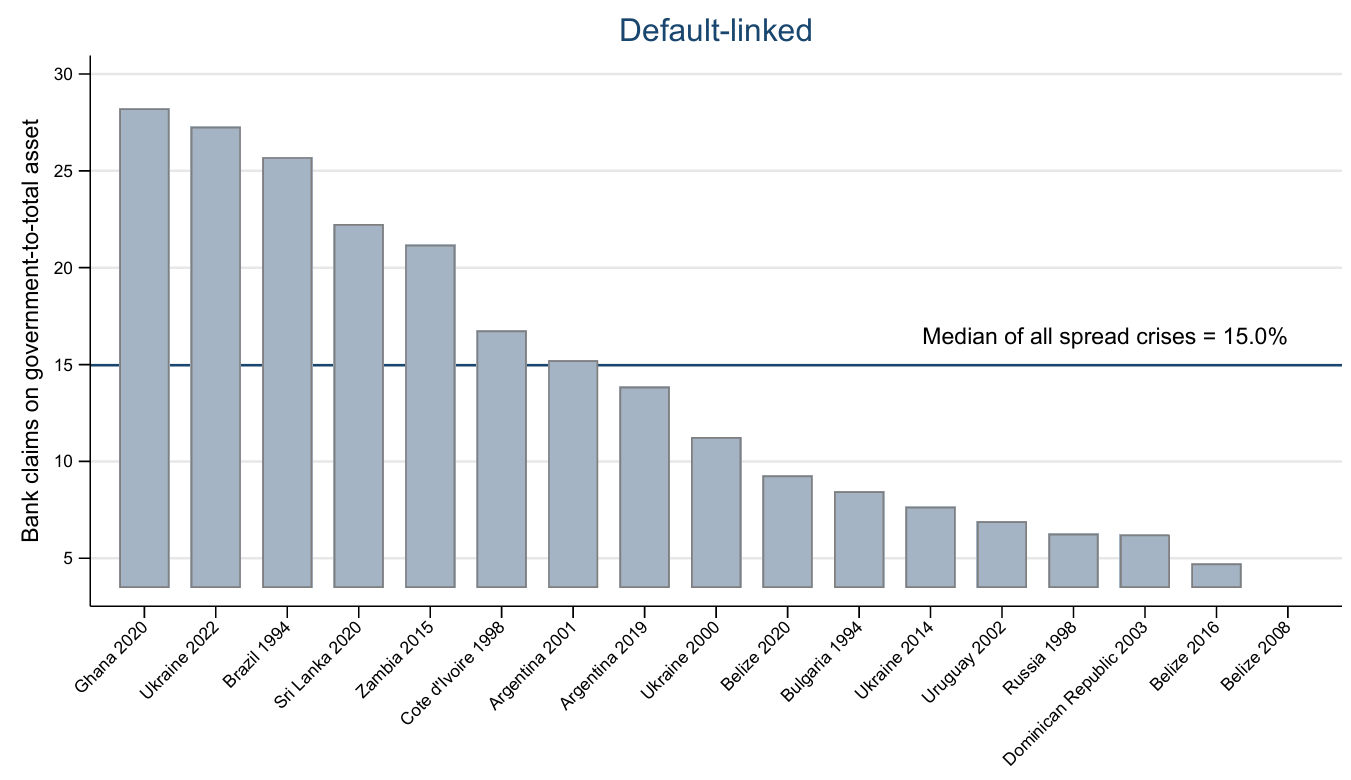
\includegraphics[width=0.95\textwidth]{figures/fig2_ols_lp.png}
\caption{OLS local projection.}
\label{fig:2}
\notes{The figure shows OLS local projection estimates. Year 1 is the
crisis onset year. The dependent variable is the cumulative log change
(GDP, investment, bank credit, real lending rate) or cumulative
percentage-point change (claims on government, FDI) from its
country-specific pre-crisis level. Non-default (blue) and default-linked
(red) onsets are each estimated in a separate regression against tranquil
years, with the rival type excluded from that regression's own sample.
Panels A--D use a balanced sample across the same crisis episodes; Panels
E--F use their own best-available sample. The shaded bands indicate each
type's own 95 percent confidence interval.}
\end{figure}

Bank credit experiences a sharp and continuously deepening decline
following a default-linked onset (red line, Panel C). Negative values
indicate the cumulative percent change in bank credit relative to its
country-specific pre-crisis level. The decline is small and not
statistically significant on impact but widens sharply from year 2 onward
and remains large and statistically significant through year 5 (blue
line, Panel C, non-default). In contrast, credit experiences a much
milder and largely insignificant decline following a non-default onset.

Claims on government rise modestly in the years immediately following a
default-linked onset, a pattern that is statistically significant only in
the first year and fades by the end of the horizon, where the two groups
are no longer distinguishable.

Investment declines in both groups following onset, with a somewhat
larger decline in the default-linked group throughout, but this gap
between the two groups is not statistically significant at any horizon.

FDI shows little movement in either group and no statistically
significant difference between them at any point in the estimation
horizon.

The real lending interest rate shows no consistent pattern between the two
groups over most of the horizon, but the default-linked group experiences
a significantly sharper decline than the non-default group at two points,
roughly a third and roughly two-thirds of the way through the horizon.

% ============================================================
\section{Augmented Inverse Probability Weighted (AIPW) Estimation}
% ============================================================

\subsection{Probit Regression on Spread Crisis Onsets}

A country's exposure to a spread crisis and decision to restructure its
debt is affected by the economic conditions that it faces, spread crisis
and restructuring being associated with negative shocks (and those
negative starting conditions can then be worsened by the spread crisis and
the restructuring itself). To attenuate that bias, we apply the augmented
inverse probability weighted (AIPW) estimation. The AIPW estimator differs
from OLS by weighting observations according to how likely they were, ex
ante, to enter each crisis category: observations that were highly
predictable candidates for a given crisis type receive a smaller weight,
and observations that were not receive a larger one, so that the
estimated cost is drawn from a distribution of observations closer to
what would have prevailed absent this predictable component of selection
(Altonji et al., 2005).

Those weights are obtained by a first-stage probit regression based on
data in the year of the start of the spread crisis and in the previous
year. The probit regression specification includes both controls and
predictors following the previous studies on AIPW estimation (Jord\'a and
Taylor, 2016; Jord\'a et al., 2020). Predictors are defined as variables
that satisfy an exclusion restriction (reported in the bottom section of
Table~\ref{tab:probit}) and influence a country's probability of entering
a spread crisis but are not influenced by that country's own spread
crisis.

Our choice of predictors is lagged: (i) the US federal funds rate; (ii) a
contagion measure constructed from the debt restructuring dummies of
other debtor countries, weighted by the geographical distances between
each debtor country and the others; (iii) years since the country's own
most recent prior default-linked spread onset. Both the US federal funds
rate and the other debtor countries' debt restructurings come from
Asonuma et al.\ (2024) and are orthogonal to country $i$'s spread crisis
type in year $t$. Years since the most recent prior default-linked spread
crisis is predetermined in year $t$.

We estimate two probit models predicting the start of a default-linked
and a non-default spread crisis, respectively, each pooled across
countries, without country fixed effects; country fixed effects enter
only the second-stage outcome model:

\begin{equation}
\label{eq:3}
\Pr\!\left(D_{i,t}^S = 1\right) = \Phi\!\left(\theta^{S\prime} X_{i,t-1} + \delta^{S\prime} Z_{i,t-1}\right),
\qquad S \in \{\text{non-default}, \text{default-linked}\}
\end{equation}

\noindent where $X_{i,t-1}$ is our baseline control set, and $Z_{i,t-1}$ is
the set of predictors defined above; $\theta^S$ and $\delta^S$ are the
coefficients. Estimating the regression yields the predicted likelihood
of each type of spread crisis, $\widehat{p}_{i,t}^S$.

\emph{[Editorial note: equation (3) was embedded as a .emf equation
object in the source document; the probit form above is reconstructed
from the surrounding prose and should be verified against the original.]}

The probit regression results are reported in Table~\ref{tab:probit}.
Predictors play a role in explaining the two types of spread crises. A
higher US federal funds rate is positively and significantly associated
with the probability of both default-linked and non-default crisis
onset, suggesting that tighter US monetary conditions are associated with
a higher likelihood of entering a spread crisis. The contagion variable is
negatively and significantly associated with the probability of
non-default crisis onset, but its coefficient is not statistically
significant for default-linked crisis onset. Years since the country's
last default-linked onset are negatively and significantly associated
with the probability of both types of crisis onset. Thus, conditional on
the other predictors, countries that have gone longer without a
default-linked crisis are less likely to experience either type of spread
crisis.

The baseline controls show limited predictive power in the non-default
specification, with none of the eight domestic macroeconomic and
financial controls statistically significant. By contrast, GDP growth,
bank credit-to-GDP, log inflation, and the nominal exchange rate are
statistically significant predictors of default-linked crisis onset. This
contrast suggests that the two types of spread crises are associated with
different underlying conditions. Non-default crisis onsets appear to be
more closely associated with external financial conditions, as captured
by the US federal funds rate and the contagion measure, whereas
default-linked onsets are more strongly associated with domestic
macroeconomic and financial conditions.

The implied areas under the ROC curve are 0.768 for non-default crises and
0.886 for default-linked crises, indicating reasonably good classification
performance in both cases. Relative to the probit specifications with
controls only, adding the three predictors increases the AUC from 0.652
to 0.768 for non-default crises and from 0.839 to 0.886 for default-linked
crises. For the non-default specification, this improvement is
statistically significant according to a formal test of equal ROC areas
(a likelihood-ratio-type test distinct from the joint-significance
chi-squared reported in Table~\ref{tab:probit}). For the default-linked
specification, the corresponding improvement is not statistically
significant. Thus, while the addition of the predictors is associated
with a sizeable improvement in classification performance for both types
of crises, only the improvement for non-default crises is statistically
established.

\begin{table}[htbp]
\centering
\caption{First-stage probit: predicting the start of a spread crisis}
\label{tab:probit}
\begin{tabular}{lcc}
\toprule
 & Non-default & Default-linked \\
 & (1) & (2) \\
\midrule
\multicolumn{3}{l}{\textit{Predictors}} \\
US federal funds rate & 19.070*** & 14.621*** \\
 & (3.473) & (5.456) \\
Contagion & $-$3.262*** & $-$1.843 \\
 & (1.145) & (1.909) \\
Years since last default-linked onset & $-$0.008** & $-$0.018** \\
 & (0.003) & (0.008) \\[4pt]
\multicolumn{3}{l}{\textit{Baseline controls}} \\
GDP growth & 0.634 & $-$6.979*** \\
 & (3.780) & (2.264) \\
Public debt-to-GDP ratio & 0.335 & 0.424 \\
 & (0.236) & (0.562) \\
Banking crisis dummy & 0.462 & 0.065 \\
 & (0.337) & (0.482) \\
Government expenditure-to-GDP ratio & $-$0.583 & $-$1.551 \\
 & (1.128) & (1.630) \\
Trade openness & $-$0.424 & 0.502 \\
 & (0.268) & (0.472) \\
Bank credit-to-GDP ratio & 0.046 & $-$2.075*** \\
 & (0.369) & (0.692) \\
Inflation & 1.265 & $-$8.200*** \\
 & (0.978) & (2.156) \\
Nominal exchange-rate & $-$0.250 & 4.821*** \\
 & (0.545) & (0.834) \\[4pt]
Chi-squared for predictors & 41.98 & 8.13 \\
$p$-value of chi-squared & 0.000 & 0.043 \\
AUROC, controls only & 0.652 & 0.839 \\
AUROC, with predictors & 0.768 & 0.886 \\
Observations & 933 & 917 \\
\bottomrule
\end{tabular}
\notes{Robust standard errors clustered by country in parentheses.
* p$<$0.10, ** p$<$0.05, *** p$<$0.01.}
\end{table}

\begin{figure}[htbp]
\centering
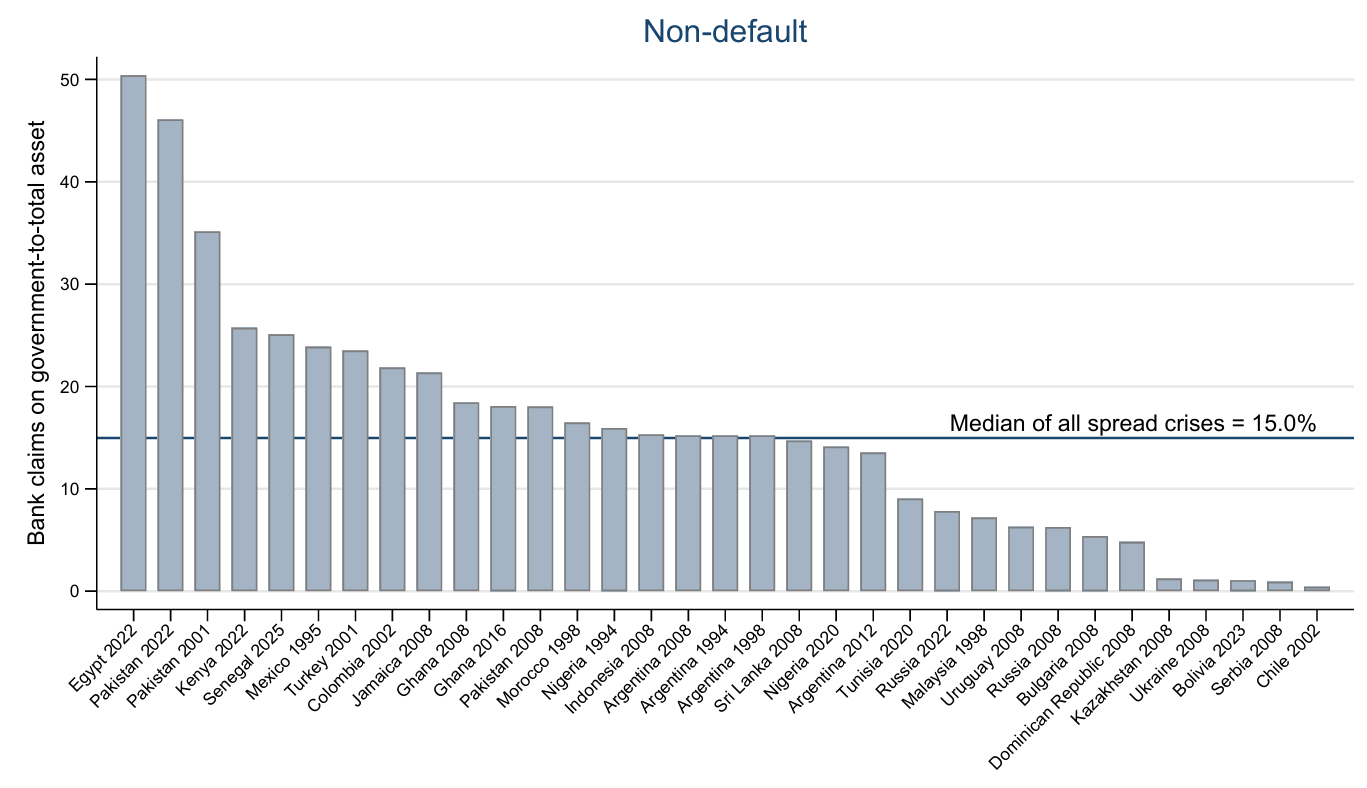
\includegraphics[width=0.8\textwidth]{figures/fig3_kernel_density.png}
\caption{Kernel density estimates.}
\label{fig:3}
\notes{The figure shows kernel density estimates of the predicted
probability of a spread crisis onset for the control group and the
treatment group, for the two types of spread crises. The numbers on the
vertical axis exceed 1 because the unit of the vertical axis is
reciprocal to the unit of the variable on the horizontal axis.
Observations with a predicted probability above 0.60 are excluded from
the density estimate; no predicted probability in this sample exceeds
approximately 0.3, which is why the plotted range does not extend
further.}
\end{figure}

\subsection{Augmented Inverse Probability Weighted (AIPW) Estimation}

We implement the AIPW estimation following Jord\'a and Taylor (2016). For
each crisis type $S \in \{\text{non-default}, \text{default-linked}\}$ and
horizon $h$, we first estimate the conditional outcome models using OLS
based on the baseline specifications in equations~(\ref{eq:1}) and
(\ref{eq:2}). These regressions yield the predicted conditional means
$\widehat{m}_1^{S,h}$ and $\widehat{m}_0^{S,h}$ corresponding to the
treated and untreated states, respectively. Second, we estimate the
probit model in equation~(\ref{eq:3}) to obtain the predicted probability
of experiencing a spread crisis of type $S$, denoted $\widehat{p}^S$.
Finally, we combine the estimated outcome models and treatment
probabilities to construct the AIPW estimator:

\begin{equation}
\label{eq:4}
\widehat{\beta}^{S,h}_{AIPW} =
\frac{1}{N}\sum_{i,t} \left[
\left( \frac{D_{i,t}^S\, y_{i,t+h}}{\widehat{p}^S_{i,t}}
     - \frac{(1-D_{i,t}^S)\, y_{i,t+h}}{1-\widehat{p}^S_{i,t}} \right)
- \frac{D_{i,t}^S - \widehat{p}^S_{i,t}}{\widehat{p}^S_{i,t}\left(1-\widehat{p}^S_{i,t}\right)}
\left[ \left(1-\widehat{p}^S_{i,t}\right)\widehat{m}_1^{S,h} + \widehat{p}^S_{i,t}\,\widehat{m}_0^{S,h} \right]
\right]
\end{equation}

\noindent where the first component of the estimator corresponds to the
inverse-probability-weighted (IPW) component, which reweights
observations according to their estimated probability of treatment. The
second component is the augmentation term, which incorporates the
predicted conditional outcomes from the OLS models. The resulting
estimator therefore combines outcome regression and inverse-probability
weighting, reducing sensitivity to misspecification of either component.

\emph{[Editorial note: equation (4) is reconstructed directly from this
project's own Stata implementation (the \texttt{\_aipw} program) rather
than from the unrenderable .emf object in the source document, and should
match the original formula exactly; please verify.]}

Figure~\ref{fig:4} reports the AIPW estimates corresponding to the
specifications presented in Table~\ref{tab:aipw}. For each crisis type,
the figure plots the estimated cumulative effect at each horizon,
together with the associated confidence interval. The estimates are
expressed as cumulative changes relative to the pre-crisis year ($t=0$).
Table~\ref{tab:aipw} reports three sets of statistical measures. First,
conventional $t$-tests assess whether the estimated coefficients are
statistically different from zero. Second, we report two complementary
tests of differences between coefficients across specifications. The
first is based on a bootstrap procedure, while the second follows the
approach proposed by Clogg et al.\ (1995). The bootstrapped results are
constructed by resampling the original data, computing the difference in
the point estimates in that bootstrapped sample, and reporting the
confidence interval for that difference based on the corresponding
percentile across 1,000 draws. These tests enable us to assess whether the
difference between estimated coefficients for the two types of
sovereign-spread crises is significantly different from zero.

\begin{figure}[htbp]
\centering
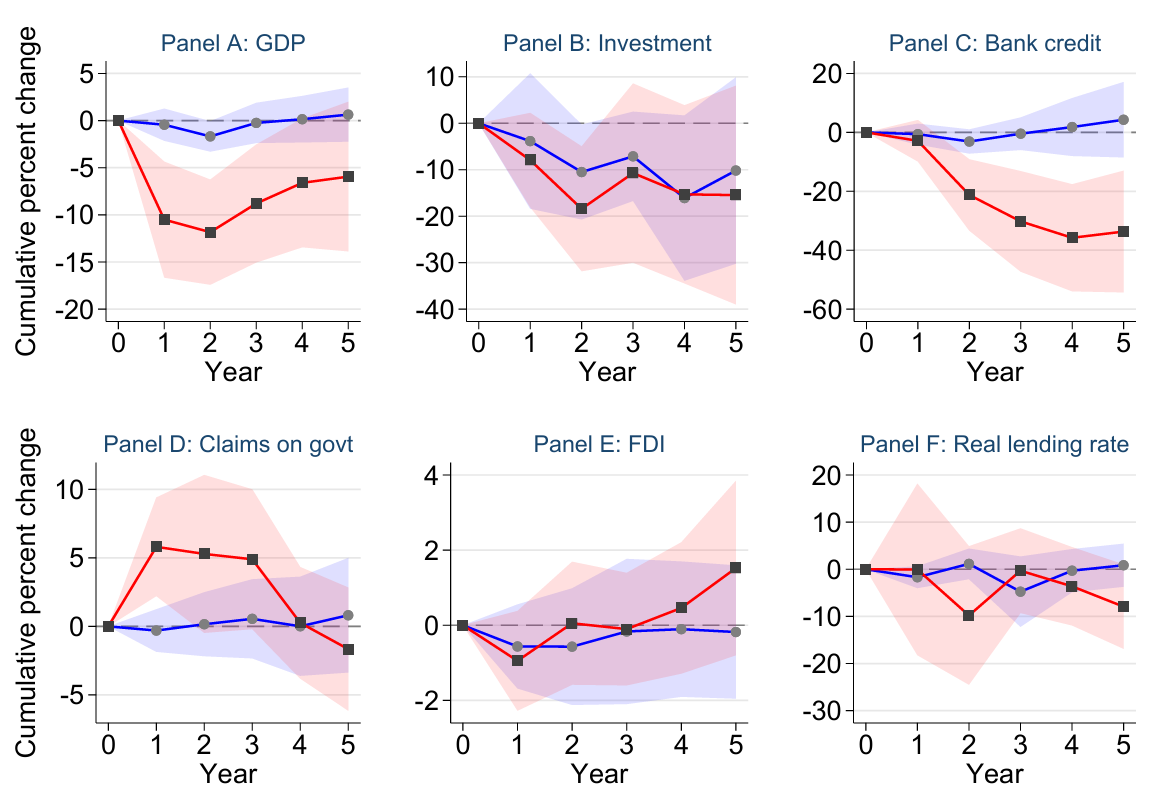
\includegraphics[width=0.95\textwidth]{figures/fig4_aipw_lp.png}
\caption{Local projections, AIPW.}
\label{fig:4}
\notes{The figure shows AIPW estimation results, based on Table~2. Year 1
is the crisis onset year. Non-default (blue) and default-linked (red)
onsets are each estimated in a separate regression against tranquil
years, with the rival type excluded from that regression's own sample.
Panels A--D (GDP, investment, bank credit, claims on government) use a
balanced sample across the same crisis episodes; Panels E--F (FDI, real
lending interest rate) use their own best-available sample, to cover as
many crisis episodes as possible. The shaded bands indicate each type's
own 95 percent confidence interval.}
\end{figure}

Following default-linked crises (red lines in Panels A--C), GDP,
investment, and bank credit exhibit large and persistent declines. By
contrast, following non-default crises (blue lines in Panels A--C), GDP
and bank credit decline more modestly and largely recover by the end of
the horizon, while the contraction in investment is of a broadly similar
magnitude to that observed following default-linked crises. The
difference in GDP growth between the two types of crises is statistically
significant over the full horizon according to the Clogg et al.\ (1995)
test and during the first two years according to the bootstrap test. For
bank credit, the difference is statistically significant under both
tests from year 2 onward, although not in the crisis year. For
investment, the Clogg et al.\ (1995) test indicates significant
differences during the first three years, whereas the bootstrap test does
not reject equality at any horizon, reflecting the relatively wide
confidence intervals around the estimated differences.

Claims on government relative to GDP increase following default-linked
crises but remain broadly unchanged following non-default crises. The
difference between the two groups is statistically significant under
both tests in the crisis year and remains significant under the Clogg et
al.\ (1995) test through year 3. The difference subsequently loses
statistical significance and becomes negative by year 5. Real lending
interest rates decline following non-default crises in most years,
whereas their response following default-linked crises is larger and
more volatile, with a marked decline from year 2 onward. The Clogg et
al.\ (1995) test indicates a statistically significant difference between
the two groups throughout the horizon, while the bootstrap test does not
reject equality at any horizon. Finally, FDI exhibits limited changes in
both groups over most of the horizon. In the final year, FDI becomes
significantly positive following default-linked crises, coinciding with a
statistically significant difference between the two groups under the
Clogg et al.\ (1995) test. However, the bootstrap test does not indicate a
statistically significant difference at any horizon.

\begin{table}[p]
\centering
\caption{AIPW estimation results}
\label{tab:aipw}
\footnotesize
\begin{tabular}{lccccc}
\toprule
\multicolumn{6}{l}{\textbf{Panel A: GDP}} \\
 & $h=1$ & $h=2$ & $h=3$ & $h=4$ & $h=5$ \\
\midrule
Non-default & $-$1.396*** & $-$2.133*** & $-$0.197 & 0.390 & 0.923 \\
 & (0.381) & (0.408) & (0.459) & (0.498) & (0.582) \\
Obs./Countries/Episodes & 640/46/20 & 640/46/20 & 640/46/20 & 640/46/20 & 640/46/20 \\
Default-linked & $-$6.093*** & $-$8.822*** & $-$6.181*** & $-$4.212*** & $-$4.479*** \\
 & (0.174) & (0.219) & (0.255) & (0.309) & (0.400) \\
Obs./Countries/Episodes & 631/46/11 & 631/46/11 & 631/46/11 & 631/46/11 & 631/46/11 \\
Difference [bootstrap 95\% CI] & [$-$8.60,$-$0.43]* & [$-$10.52,$-$0.35]* & [$-$10.75,2.27] & [$-$11.01,3.63] & [$-$15.03,3.31] \\
(Clogg $z$) & ($-$11.22***) & ($-$14.43***) & ($-$11.41***) & ($-$7.86***) & ($-$7.65***) \\
\addlinespace
\multicolumn{6}{l}{\textbf{Panel B: Investment}} \\
 & $h=1$ & $h=2$ & $h=3$ & $h=4$ & $h=5$ \\
\midrule
Non-default & $-$4.825*** & $-$9.680*** & $-$5.698*** & $-$13.695*** & $-$7.506*** \\
 & (1.567) & (1.691) & (1.399) & (1.985) & (2.332) \\
Obs./Countries/Episodes & 640/46/20 & 640/46/20 & 640/46/20 & 640/46/20 & 640/46/20 \\
Default-linked & $-$8.761*** & $-$17.684*** & $-$9.832*** & $-$13.818*** & $-$12.406*** \\
 & (0.560) & (0.810) & (1.122) & (1.150) & (1.294) \\
Obs./Countries/Episodes & 631/46/11 & 631/46/11 & 631/46/11 & 631/46/11 & 631/46/11 \\
Difference [bootstrap 95\% CI] & [$-$18.98,14.71] & [$-$26.19,9.56] & [$-$30.51,16.46] & [$-$26.77,26.87] & [$-$38.87,28.58] \\
(Clogg $z$) & ($-$2.37**) & ($-$4.27***) & ($-$2.31**) & ($-$0.05) & ($-$1.84*) \\
\addlinespace
\multicolumn{6}{l}{\textbf{Panel C: Bank credit}} \\
 & $h=1$ & $h=2$ & $h=3$ & $h=4$ & $h=5$ \\
\midrule
Non-default & $-$1.056** & $-$3.021*** & 0.222 & 3.162*** & 6.791*** \\
 & (0.444) & (0.676) & (0.838) & (1.175) & (1.446) \\
Obs./Countries/Episodes & 627/46/19 & 627/46/19 & 627/46/19 & 627/46/19 & 627/46/19 \\
Default-linked & $-$0.782 & $-$23.024*** & $-$36.794*** & $-$41.945*** & $-$39.879*** \\
 & (0.483) & (0.708) & (1.176) & (1.230) & (1.327) \\
Obs./Countries/Episodes & 619/46/11 & 619/46/11 & 619/46/11 & 619/46/11 & 619/46/11 \\
Difference [bootstrap 95\% CI] & [$-$9.15,8.08] & [$-$29.55,$-$6.15]* & [$-$51.06,$-$6.89]* & [$-$55.49,$-$8.77]* & [$-$59.90,$-$7.17]* \\
(Clogg $z$) & (0.42) & ($-$20.43***) & ($-$25.63***) & ($-$26.52***) & ($-$23.78***) \\
\bottomrule
\end{tabular}
\end{table}

\begin{table}[p]
\centering
\ContinuedFloat
\footnotesize
\begin{tabular}{lccccc}
\multicolumn{6}{l}{\textbf{Panel D: Bank claims on government}} \\
 & $h=1$ & $h=2$ & $h=3$ & $h=4$ & $h=5$ \\
\midrule
Non-default & $-$0.707*** & $-$0.484 & $-$0.287 & $-$0.833* & $-$0.384 \\
 & (0.222) & (0.325) & (0.377) & (0.457) & (0.566) \\
Obs./Countries/Episodes & 639/46/20 & 639/46/20 & 639/46/20 & 639/46/20 & 639/46/20 \\
Default-linked & 6.665*** & 5.754*** & 4.895*** & $-$0.268 & $-$2.605*** \\
 & (0.193) & (0.229) & (0.236) & (0.254) & (0.300) \\
Obs./Countries/Episodes & 630/46/11 & 630/46/11 & 630/46/11 & 630/46/11 & 630/46/11 \\
Difference [bootstrap 95\% CI] & [0.66,9.99]* & [$-$1.45,10.45] & [$-$2.61,8.64] & [$-$6.27,5.44] & [$-$9.10,4.49] \\
(Clogg $z$) & (25.06***) & (15.70***) & (11.66***) & (1.08) & ($-$3.47***) \\
\addlinespace
\multicolumn{6}{l}{\textbf{Panel E: FDI}} \\
 & $h=1$ & $h=2$ & $h=3$ & $h=4$ & $h=5$ \\
\midrule
Non-default & $-$0.639** & $-$0.435 & $-$0.017 & 0.131 & $-$0.066 \\
 & (0.265) & (0.327) & (0.356) & (0.335) & (0.341) \\
Obs./Countries/Episodes & 893/47/30 & 857/47/30 & 822/47/30 & 788/47/28 & 750/47/25 \\
Default-linked & $-$0.925*** & 0.182 & 0.004 & 0.658** & 1.824*** \\
 & (0.249) & (0.315) & (0.305) & (0.315) & (0.344) \\
Obs./Countries/Episodes & 879/47/16 & 843/47/16 & 808/47/16 & 775/47/15 & 740/47/15 \\
Difference [bootstrap 95\% CI] & [$-$1.76,1.37] & [$-$1.94,2.70] & [$-$1.79,2.69] & [$-$2.42,2.62] & [$-$1.78,4.42] \\
(Clogg $z$) & ($-$0.79) & (1.36) & (0.05) & (1.15) & (3.90***) \\
\addlinespace
\multicolumn{6}{l}{\textbf{Panel F: Real lending rate}} \\
 & $h=1$ & $h=2$ & $h=3$ & $h=4$ & $h=5$ \\
\midrule
Non-default & $-$1.498*** & 0.969** & $-$4.285*** & $-$0.456 & 0.065 \\
 & (0.301) & (0.463) & (0.799) & (0.387) & (0.395) \\
Obs./Countries/Episodes & 658/39/19 & 626/39/19 & 594/39/19 & 558/39/14 & 523/38/14 \\
Default-linked & 1.573 & $-$8.890*** & $-$1.712*** & $-$4.598*** & $-$10.006*** \\
 & (1.078) & (1.033) & (0.637) & (0.702) & (0.608) \\
Obs./Countries/Episodes & 649/39/10 & 617/39/10 & 584/39/9 & 553/38/9 & 517/37/8 \\
Difference [bootstrap 95\% CI] & [$-$13.44,20.60] & [$-$23.03,3.78] & [$-$8.61,14.87] & [$-$13.37,6.28] & [$-$19.60,2.20] \\
(Clogg $z$) & (2.74***) & ($-$8.71***) & (2.52**) & ($-$5.17***) & ($-$13.89***) \\
\bottomrule
\end{tabular}
\notes{The table shows the AIPW estimation results. $h=1$ is the crisis
onset year. Non-default and default-linked crises are estimated in
separate regressions, each vs.\ tranquil years with the rival type
dropped from that regression's own sample. Panels A--D are estimated on a
balanced sample (the same episodes across all four panels); FDI and the
real lending rate use their own best-available sample to cover as many
episodes as possible. Level standard errors (in parentheses) are the
analytic (unclustered influence-function) SE; single-tier stars test each
coefficient against zero. The bracketed 95\% CI on each difference
(default $-$ non-default) is a paired row-bootstrap (1,000 draws), the
governing test (* excludes zero); cells with fewer than 50 valid draws are
not reported. The Clogg $z$ below each CI (own $p$-value, 3-tier stars) is
a permissive companion statistic assuming independence between the two
crisis types; where the two disagree, the bootstrap governs.
* p$<$0.10, ** p$<$0.05, *** p$<$0.01.}
\end{table}

\clearpage

% ============================================================
\section{Role of the Sovereign-Bank Nexus}
% ============================================================

The relationship between the financial health of the public sector and
the domestic banking system, often termed the sovereign-bank nexus, is a
critical area of analysis for macrofinancial stability. Excessive
interdependence can become perilous, especially when sovereigns
increasingly rely on domestic banks for financing amid rising and
increasingly unsustainable public debt. Distress in one sector can
propagate and amplify stress in the other, potentially creating adverse
feedback loops (Dell'Ariccia et al., 2018). Banks often hold large
portfolios of sovereign bonds, while governments implicitly or explicitly
backstop banks in crisis. This creates a two-way feedback loop: fiscal
distress can weaken banks, and banking crises can worsen public finances.
Furthermore, a strong nexus can create vulnerabilities even absent a
default. It can crowd out credit to the private sector (Broner et al.,
2014) and, in an environment of rising interest rates, expose banks to
potential capital losses (Copestake et al., 2023).

The sovereign debt crisis in the euro area provided clear evidence of the
potential for these feedback mechanisms to amplify financial and fiscal
distress. More recently, the COVID-19 pandemic further increased public
debt levels and was accompanied by a substantial rise in domestic banks'
holdings of sovereign debt, particularly in emerging market and
developing economies (Deghi et al., 2022). Against a backdrop of tighter
global financial conditions and increased refinancing pressures, these
developments have renewed attention to the sovereign-bank nexus and its
implications for financial stability.

Recent evidence suggests that these vulnerabilities have strengthened in
the post-pandemic period. Wezel, Barrail, and Dehmej (2026) document a
particularly pronounced strengthening of the sovereign-bank nexus in
Sub-Saharan Africa and the Middle East and Central Asia. They identify
public debt levels, deposit rates, and non-performing loans as important
correlates of banks' sovereign exposure. Their results further indicate
that higher sovereign refinancing needs are associated with larger bank
holdings of government debt, particularly in countries with a substantial
presence of state-owned banks. These findings highlight the importance of
domestic banks as a potential transmission channel of sovereign stress,
particularly in emerging and developing economies where sovereign
financing needs can be closely intertwined with domestic financial
conditions.

Building on this literature, we examine whether the pre-crisis exposure
of domestic banks to the sovereign is associated with heterogeneous
effects of sovereign spread crises on the domestic economy. We focus on
GDP, domestic bank credit to the private sector, and investment, which
together allow us to examine whether differences in sovereign exposure
are reflected in the transmission of sovereign stress to economic
activity through the domestic financial system.

This design supports two complementary comparisons: whether outcomes
differ between high- and low-exposure banking sectors within a given
resolution type, and whether the gap between default-linked and
non-default crises itself depends on pre-crisis exposure. The first
isolates the direct amplification effect of the nexus; the second asks
whether a tight sovereign-bank nexus sharpens the distinction between
resolution strategies. We report both, since the evidence discussed below
does not point to the same answer for each.

We measure the sovereign-bank nexus using banks' claims on government as
a share of total bank assets, lagged by one year relative to crisis
onset. This measure captures the extent to which the domestic banking
system is directly exposed to sovereign credit risk prior to the crisis
and therefore closely corresponds to the balance-sheet mechanism
described above. We classify crisis onsets into high- and low-nexus
groups according to the sample median of this ratio across all onset
observations. Figure~\ref{fig:5} reports the distribution of the measure
separately for non-default and default-linked crisis onsets. The median
across the full onset sample is 14.96\%, resulting in an approximately
even split between high- and low-nexus observations, with 25 onsets in
each group. The classification nevertheless differs across crisis types:
non-default crises are more frequently classified as high-nexus, whereas
default-linked crises are more frequently classified as low-nexus. The
average claims-on-government ratio is below 7 percent of bank assets in
the low-nexus group and above 23 percent in the high-nexus group. The two
groups are not concentrated in an obviously distinct set of countries,
although differences in income composition suggest that the nexus measure
may also capture broader differences in financial and economic
development. We therefore interpret the resulting split as a measure of
sovereign-bank exposure rather than as a cleanly exogenous classification.

\begin{figure}[htbp]
\centering
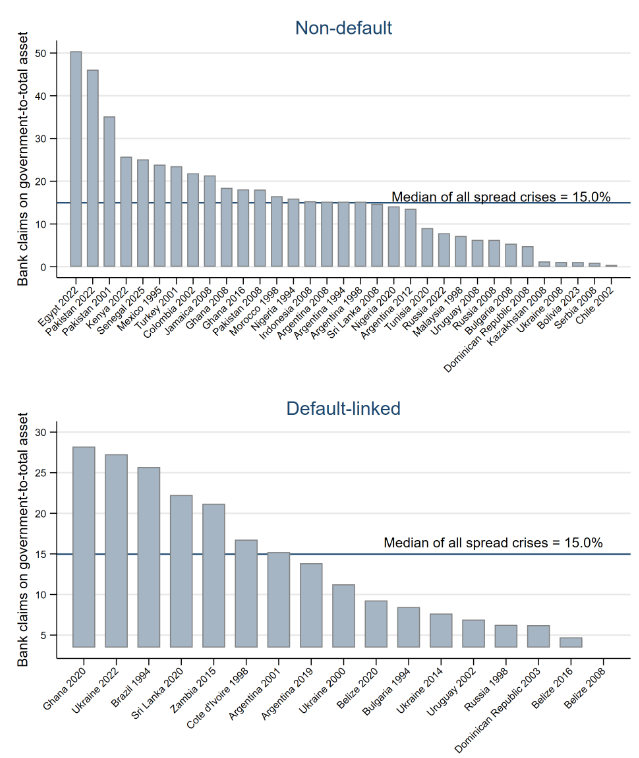
\includegraphics[width=0.75\textwidth]{figures/fig5_nexus_distribution.png}
\caption{Bank sovereign nexus in the pre-crisis year, crises with and without default.}
\label{fig:5}
\end{figure}

To assess whether the size of the sovereign-bank nexus is associated with
heterogeneous effects across type of crisis, we interact the spread
crisis type indicator with the high- and low-nexus classifications
within the same local-projection framework used throughout the analysis:

\begin{equation}
\label{eq:5}
y_{i,t+h} - y_{i,t-1} = \alpha_i^{S,h}
  + \beta^{S,h}_{high}\, D_{i,t}^{S}\, \mathrm{High}_{i,t-1}
  + \beta^{S,h}_{low}\, D_{i,t}^{S}\, \left(1-\mathrm{High}_{i,t-1}\right)
  + \Gamma^{S,h\prime} X_{i,t-1} + \varepsilon_{i,t+h}^{S}
\end{equation}

\noindent where $\mathrm{High}_{i,t-1}$ is a dummy equal to one if country
$i$'s sovereign-bank nexus is large in year $t-1$ and zero otherwise,
interacted with the crisis-type dummy $D_{i,t}^S$; $\beta^{S,h}_{high}$
and $\beta^{S,h}_{low}$ are the coefficients of interest, capturing the
impact of a crisis of type $S$ when the banking sector's sovereign
exposure is, respectively, large or small; $\alpha_i^{S,h}$ denotes
country fixed effects; and $X_{i,t-1}$ is the same vector of controls
used throughout.

\emph{[Editorial note: the unlabeled interaction equation preceding
Figures 6--7 was likewise embedded as a .emf object; the form above is
reconstructed from the surrounding prose.]}

As in the baseline AIPW analysis, we estimate the local-projection
specification separately by spread crisis type and sovereign-bank nexus,
yielding four sets of estimates for each outcome. Figures~\ref{fig:6}
and~\ref{fig:7} present the results in two complementary ways.
Figure~\ref{fig:6} compares high- and low-nexus countries within each
type, while Figure~\ref{fig:7} compares non-default and default-linked
crises within each nexus group. Conventional $t$-tests assess whether the
estimated effects differ from zero, while differences across groups are
evaluated using both paired bootstrap tests and the test proposed by
Clogg et al.\ (1995).

The results do not indicate that a larger pre-crisis sovereign-bank nexus
systematically amplifies the costs of non-default crises. For GDP
following non-default crises, the estimated response is in fact more
muted in the high-nexus group (orange line), which remains close to its
pre-crisis path throughout the horizon, whereas the low-nexus group
(green line) experiences a temporary decline that gradually dissipates.
The difference between the two groups reaches statistical significance
only at $h=1$, with the high-nexus group's response essentially flat that
year against the low-nexus group's initial decline; at longer horizons the
gap is not statistically significant. A similar pattern is observed for
investment following non-default crises, with somewhat more persistent
contractions in the low-nexus group, but the difference between high- and
low-nexus countries is not statistically significant at any horizon.
Bank credit shows no comparably clean pattern following non-default
crises: the high-nexus group's response is smaller than the low-nexus
group's at some horizons but not others, and swings sharply positive by
$h=5$; here too, the difference between the two groups is not
statistically significant at any horizon. Thus, while the estimates point
towards a potentially more limited response among high-nexus countries
following non-default crises, the evidence does not establish a
systematic or persistent attenuation effect.

\begin{figure}[htbp]
\centering
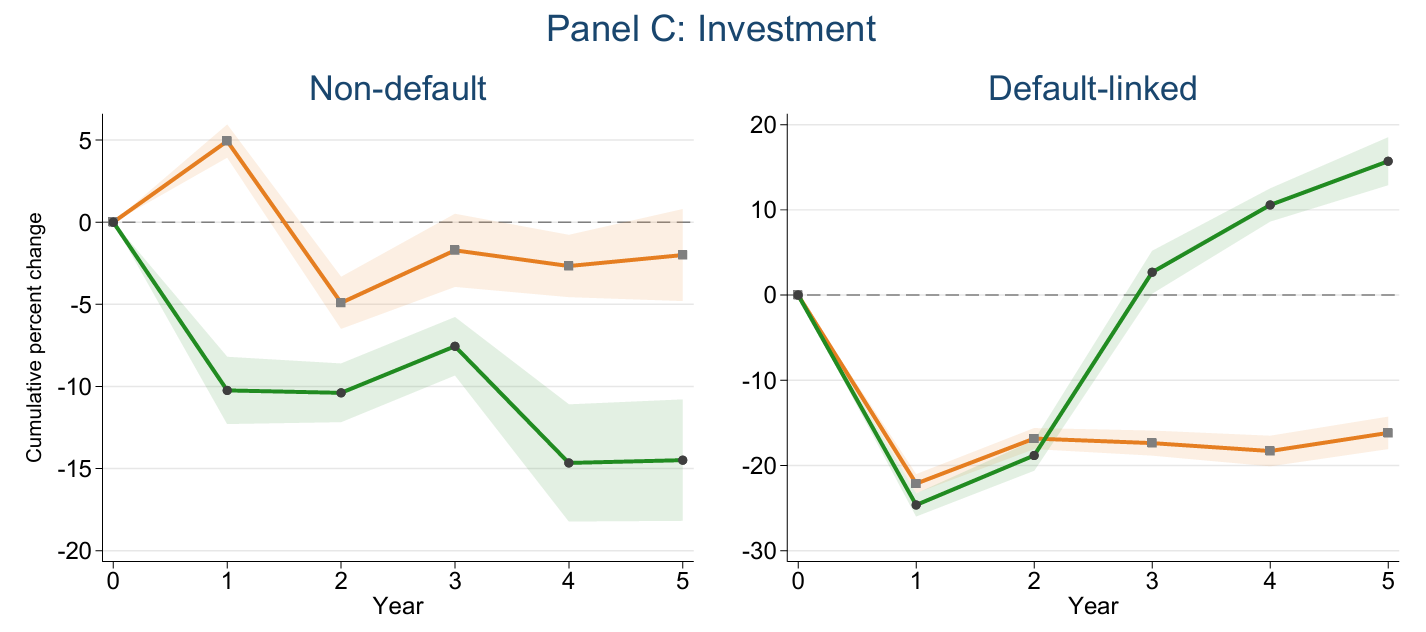
\includegraphics[width=0.95\textwidth]{figures/fig6_aipw_by_crisis_type.png}
\caption{AIPW estimation by type of crisis, high or low pre-crisis sovereign-bank nexus.}
\label{fig:6}
\notes{The figure shows AIPW estimation results for GDP, bank credit,
investment, and bank claims on government (Panels A--D), separately for
non-default crises and default-linked crises. Year 1 is the crisis onset
year. Within each type of crisis, high-nexus (orange) and low-nexus
(green) countries are each estimated in a separate regression against
tranquil years, with the rival type excluded from that regression's own
sample. The nexus is measured as bank claims on government relative to
bank assets in the year before the crisis, or the country mean when the
pre-crisis value is unavailable; countries are split into two groups
based on the sample median of this measure across all crisis onsets. The
shaded bands indicate each group's own 95 percent confidence interval,
computed from the analytic standard error.}
\end{figure}

The contrast with default-linked crises is more pronounced. GDP declines
substantially following default-linked crises in both nexus groups, but
the response is more persistent among high-nexus countries (orange line).
In the low-nexus group (green line), the initial decline gradually
reverses over the subsequent years, whereas GDP remains substantially
below its pre-crisis path in the high-nexus group throughout the
five-year horizon. The difference between high- and low-nexus countries
within the default-linked group is nevertheless not statistically
significant. However, when comparing crisis types within each nexus
group, the gap between default-linked and non-default crises is larger
and more persistent among high-nexus countries. This pattern suggests
that the sovereign-bank nexus may be more relevant for the persistence of
output losses when sovereign distress leads to a default or
restructuring, although the evidence does not establish a statistically
significant amplification effect of the nexus itself.

The dynamics of investment and bank credit are broadly consistent with
the GDP results but provide weaker statistical evidence. Following
default-linked crises, investment declines more persistently in the
high-nexus group (orange line), while the low-nexus group's (green line)
contraction gradually reverses and turns markedly positive by the later
horizons. Bank credit shows a more complicated pattern following
default-linked crises. The high-nexus group contracts immediately, with
the largest decline early in the horizon before partially recovering by
the later years. The low-nexus group's response is instead significantly
positive in the crisis year itself, before turning sharply negative from
year 2 onward and remaining large through year 5. Most of the
corresponding differences between high- and low-nexus groups are not
statistically significant. The only statistically significant difference
between the high- and low-nexus groups is observed for investment
following default-linked crises. At that horizon, the estimated response
is markedly positive in the low-nexus group, while remaining
substantially negative in the high-nexus group.

\begin{figure}[htbp]
\centering
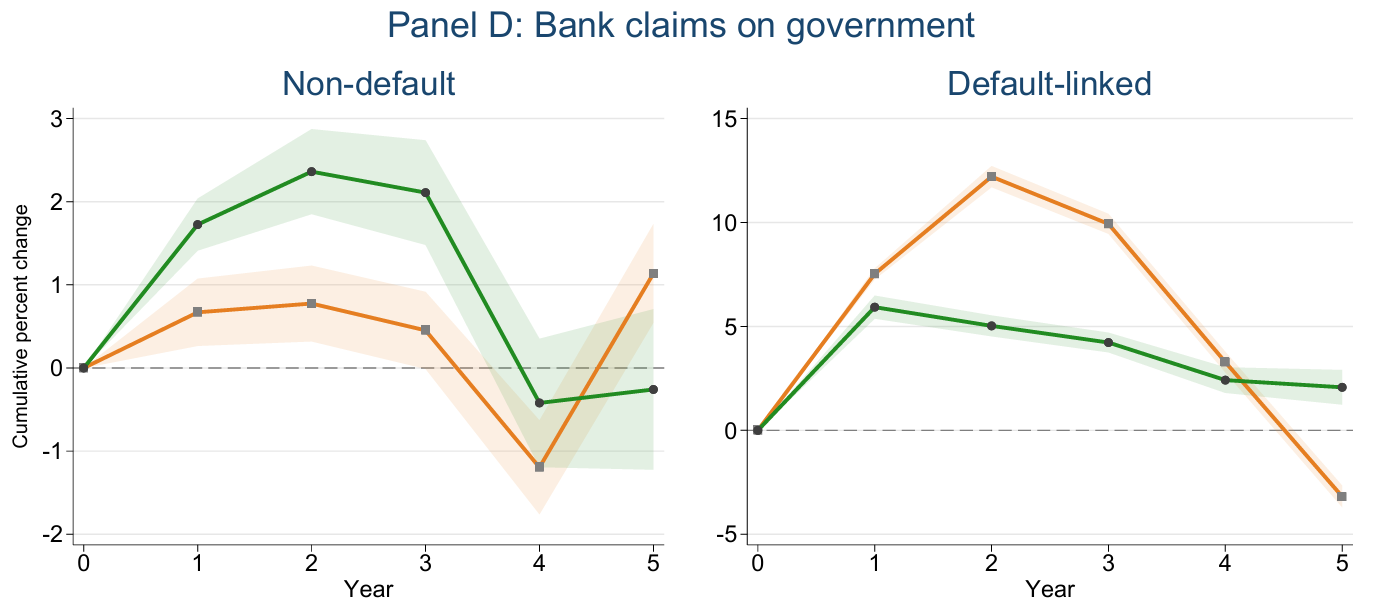
\includegraphics[width=0.95\textwidth]{figures/fig7_aipw_by_nexus.png}
\caption{AIPW estimation by pre-crisis sovereign-bank nexus, non-default or default-linked crises.}
\label{fig:7}
\notes{The figure shows AIPW estimation results for GDP, bank credit,
investment, and bank claims on government (Panels A--D), separately for
countries with a high pre-crisis sovereign-bank nexus and countries with
a low pre-crisis sovereign-bank nexus. Year 1 is the crisis onset year.
Within each nexus group, non-default (blue) and default-linked (red)
crises are each estimated in a separate regression against tranquil
years, with the rival type excluded from that regression's own sample.
The nexus is measured as bank claims on government relative to bank
assets in the year before the crisis, or the country mean when the
pre-crisis value is unavailable; countries are split into two groups
based on the sample median of this measure across all crisis onsets. The
shaded bands indicate each group's own 95 percent confidence interval,
computed from the analytic standard error.}
\end{figure}

The clearest statistically significant difference involving the
sovereign-bank nexus concerns claims on government, although it arises
from a different comparison than for the other outcomes. The difference
between high- and low-nexus countries following default-linked crises is
not statistically significant at any horizon. Instead, the significant
result comes from comparing crisis types within the high-nexus group:
claims on government increase significantly more following default-linked
crises (red line) than following non-default crises (blue line) at
horizons 2 and 3. Within the low-nexus group, the corresponding
differences are not statistically significant at any horizon. The
estimated trajectories also show a descriptively larger increase in
claims on government among high-nexus countries in years 2 and 3
following default-linked crises. This increase subsequently fades, while
the rise in the low-nexus group is smaller and more evenly distributed
over the horizon. These patterns suggest that the evolution of banks'
claims on government may differ across crisis types, particularly among
countries with greater pre-crisis sovereign exposure. However, the
absence of statistically significant differences between the high- and
low-nexus groups means that the estimates do not establish that greater
initial exposure is associated with a larger subsequent accumulation of
government claims. The results are therefore consistent with, but do not
independently establish, a sovereign-bank transmission mechanism.

\begin{landscape}
\begin{table}[p]
\centering
\caption{AIPW estimation results with high or low nexus}
\label{tab:nexus}
\footnotesize
\begin{tabular}{lccccc}
\toprule
\multicolumn{6}{l}{\textbf{Panel A: GDP}} \\
 & $h=1$ & $h=2$ & $h=3$ & $h=4$ & $h=5$ \\
\midrule
Default-linked, high nexus & $-$17.85* & $-$18.98* & $-$18.53* & $-$17.68* & $-$16.68* \\
Obs./Countries/Episodes & 907/47/7 & 879/47/7 & 843/47/7 & 809/47/7 & 776/47/7 \\
Default-linked, low nexus & $-$7.72* & $-$9.11* & $-$3.18* & 1.22* & 3.37* \\
Obs./Countries/Episodes & 909/47/10 & 881/47/10 & 845/47/10 & 811/47/10 & 778/47/10 \\
Non-default, high nexus & 0.75* & $-$0.93* & $-$0.66* & 0.65* & 0.21 \\
Obs./Countries/Episodes & 914/47/18 & 886/47/18 & 849/47/18 & 815/47/18 & 782/47/18 \\
Non-default, low nexus & $-$2.87* & $-$3.09* & $-$0.86* & $-$0.71 & 0.95* \\
Obs./Countries/Episodes & 915/47/15 & 887/47/15 & 851/47/15 & 817/47/15 & 783/47/15 \\
\addlinespace
Default(High)$-$Default(Low) & [$-$18.9,4.9] & [$-$21.4,6.5] & [$-$24.4,2.2] & [$-$29.0,2.2] & [$-$32.6,1.4] \\
(Clogg $z$) & ($-$24.15***) & ($-$22.85***) & ($-$33.56***) & ($-$36.07***) & ($-$32.11***) \\
Non-default(High)$-$Non-default(Low) & [0.0,6.9]* & [$-$0.9,5.7] & [$-$4.3,3.8] & [$-$4.8,6.3] & [$-$7.5,6.6] \\
(Clogg $z$) & (13.95***) & (7.49***) & (0.54) & (2.76***) & ($-$1.27) \\
Default(High)$-$Non-default(High) & [$-$20.8,$-$3.4]* & [$-$17.5,$-$1.6]* & [$-$17.4,1.2] & [$-$19.9,4.5] & [$-$18.3,4.6] \\
(Clogg $z$) & ($-$30.84***) & ($-$26.30***) & ($-$23.08***) & ($-$18.46***) & ($-$13.47***) \\
Default(Low)$-$Non-default(Low) & [$-$10.3,$-$0.1]* & [$-$12.1,2.1] & [$-$9.5,6.3] & [$-$9.5,10.1] & [$-$13.7,10.7] \\
(Clogg $z$) & ($-$11.47***) & ($-$11.54***) & ($-$3.98***) & (1.63) & (0.80) \\
\bottomrule
\end{tabular}

\vspace{6pt}
\begin{tabular}{lccccc}
\toprule
\multicolumn{6}{l}{\textbf{Panel B: Bank credit}} \\
 & $h=1$ & $h=2$ & $h=3$ & $h=4$ & $h=5$ \\
\midrule
Default-linked, high nexus & $-$16.32* & $-$32.22* & $-$34.35* & $-$13.22* & $-$3.28* \\
Obs./Countries/Episodes & 775/47/7 & 737/47/7 & 700/47/7 & 537/47/7 & 506/47/7 \\
Default-linked, low nexus & 7.24* & $-$25.13* & $-$49.71* & $-$47.95* & $-$39.65* \\
Obs./Countries/Episodes & 741/47/10 & 703/47/10 & 666/47/10 & 630/47/10 & 592/47/10 \\
Non-default, high nexus & $-$2.28* & $-$5.02* & $-$4.75* & $-$0.15 & 18.38* \\
Obs./Countries/Episodes & 780/47/18 & 741/47/18 & 703/47/18 & 667/47/18 & 627/47/18 \\
Non-default, low nexus & $-$0.90* & $-$7.64* & $-$10.36* & $-$2.67* & $-$6.29* \\
Obs./Countries/Episodes & 780/47/15 & 742/47/15 & 705/47/15 & 668/47/15 & 630/47/15 \\
\addlinespace
Default(High)$-$Default(Low) & [$-$31.3,7.2] & [$-$37.4,28.5] & [$-$41.0,58.7] & [$-$19.5,87.9] & [$-$21.6,114.9] \\
(Clogg $z$) & ($-$48.88***) & ($-$8.20***) & (12.31***) & (26.25***) & (24.73***) \\
Non-default(High)$-$Non-default(Low) & [$-$9.5,7.2] & [$-$11.6,14.6] & [$-$17.9,22.0] & [$-$21.7,21.9] & [$-$8.8,44.6] \\
(Clogg $z$) & ($-$2.35**) & (3.18***) & (4.66***) & (1.82*) & (17.25***) \\
Default(High)$-$Non-default(High) & [$-$22.8,14.0] & [$-$47.8,15.8] & [$-$51.8,28.2] & [$-$40.9,32.1] & [$-$61.4,133.9] \\
(Clogg $z$) & ($-$12.24***) & ($-$14.87***) & ($-$8.56***) & ($-$3.43***) & ($-$8.60***) \\
Default(Low)$-$Non-default(Low) & [$-$10.0,15.2] & [$-$32.8,7.6] & [$-$59.0,15.7] & [$-$56.0,13.0] & [$-$37.5,22.7] \\
(Clogg $z$) & (10.55***) & ($-$16.08***) & ($-$19.79***) & ($-$19.75***) & ($-$8.88***) \\
\bottomrule
\end{tabular}
\end{table}
\end{landscape}

\begin{landscape}
\begin{table}[p]
\centering
\ContinuedFloat
\footnotesize
\begin{tabular}{lccccc}
\toprule
\multicolumn{6}{l}{\textbf{Panel C: Investment}} \\
 & $h=1$ & $h=2$ & $h=3$ & $h=4$ & $h=5$ \\
\midrule
Default-linked, high nexus & $-$22.13* & $-$16.84* & $-$17.37* & $-$18.30* & $-$16.17* \\
Obs./Countries/Episodes & 890/46/7 & 862/46/7 & 826/46/7 & 792/46/7 & 759/46/7 \\
Default-linked, low nexus & $-$24.63* & $-$18.83* & 2.68* & 10.57* & 15.71* \\
Obs./Countries/Episodes & 892/46/10 & 864/46/10 & 828/46/10 & 794/46/10 & 761/46/10 \\
Non-default, high nexus & 4.94* & $-$4.91* & $-$1.71 & $-$2.67* & $-$2.00 \\
Obs./Countries/Episodes & 897/46/18 & 869/46/18 & 832/46/18 & 798/46/18 & 765/46/18 \\
Non-default, low nexus & $-$10.24* & $-$10.39* & $-$7.55* & $-$14.66* & $-$14.49* \\
Obs./Countries/Episodes & 898/46/15 & 870/46/15 & 834/46/15 & 800/46/15 & 766/46/15 \\
\addlinespace
Default(High)$-$Default(Low) & [$-$23.4,32.8] & [$-$23.2,21.2] & [$-$42.4,8.2] & [$-$65.5,3.7] & [$-$70.9,$-$2.0]* \\
(Clogg $z$) & (2.84***) & (1.81*) & ($-$13.57***) & ($-$21.54***) & ($-$18.49***) \\
Non-default(High)$-$Non-default(Low) & [$-$0.7,28.7] & [$-$8.4,19.1] & [$-$12.5,21.6] & [$-$14.9,34.7] & [$-$21.3,44.5] \\
(Clogg $z$) & (13.09***) & (4.52***) & (4.03***) & (5.83***) & (5.29***) \\
Default(High)$-$Non-default(High) & [$-$29.7,6.9] & [$-$26.7,16.2] & [$-$36.4,23.1] & [$-$47.9,33.7] & [$-$47.8,28.5] \\
(Clogg $z$) & ($-$12.83***) & ($-$1.52) & ($-$4.02***) & ($-$5.69***) & ($-$3.33***) \\
Default(Low)$-$Non-default(Low) & [$-$33.7,13.0] & [$-$23.6,12.1] & [$-$17.2,26.1] & [$-$8.7,57.2] & [$-$2.0,68.6] \\
(Clogg $z$) & ($-$9.54***) & ($-$6.48***) & (5.46***) & (9.84***) & (11.74***) \\
\bottomrule
\end{tabular}

\vspace{6pt}
\begin{tabular}{lccccc}
\toprule
\multicolumn{6}{l}{\textbf{Panel D: Bank claims on government}} \\
 & $h=1$ & $h=2$ & $h=3$ & $h=4$ & $h=5$ \\
\midrule
Default-linked, high nexus & 7.53* & 12.21* & 9.93* & 3.28* & $-$3.18* \\
Obs./Countries/Episodes & 863/47/7 & 824/47/7 & 787/47/7 & 751/47/7 & 586/47/7 \\
Default-linked, low nexus & 5.93* & 5.03* & 4.23* & 2.42* & 2.07* \\
Obs./Countries/Episodes & 866/47/10 & 827/47/10 & 790/47/10 & 754/47/10 & 717/47/10 \\
Non-default, high nexus & 0.67* & 0.78* & 0.45 & $-$1.20* & 1.14* \\
Obs./Countries/Episodes & 871/47/18 & 831/47/18 & 793/47/18 & 757/47/18 & 718/47/18 \\
Non-default, low nexus & 1.72* & 2.36* & 2.11* & $-$0.42 & $-$0.26 \\
Obs./Countries/Episodes & 871/47/15 & 832/47/15 & 795/47/15 & 758/47/15 & 721/47/15 \\
\addlinespace
Default(High)$-$Default(Low) & [$-$6.8,7.9] & [$-$4.3,19.4] & [$-$1.7,12.9] & [$-$9.2,8.4] & [$-$16.9,8.0] \\
(Clogg $z$) & (5.12***) & (19.70***) & (16.60***) & (2.15**) & ($-$10.49***) \\
Non-default(High)$-$Non-default(Low) & [$-$4.0,3.1] & [$-$6.2,3.4] & [$-$6.8,3.1] & [$-$8.7,5.7] & [$-$9.6,8.6] \\
(Clogg $z$) & ($-$4.05***) & ($-$4.54***) & ($-$4.16***) & ($-$1.59) & (2.41**) \\
Default(High)$-$Non-default(High) & [$-$1.3,9.3] & [0.1,26.2]* & [0.8,18.5]* & [$-$7.0,11.8] & [$-$16.4,8.8] \\
(Clogg $z$) & (11.14***) & (21.65***) & (20.16***) & (10.85***) & ($-$3.35***) \\
Default(Low)$-$Non-default(Low) & [$-$2.5,10.5] & [$-$4.2,7.3] & [$-$5.9,5.7] & [$-$8.2,10.5] & [$-$11.5,11.3] \\
(Clogg $z$) & (8.08***) & (4.30***) & (4.78***) & (6.16***) & (3.45***) \\
\bottomrule
\end{tabular}
\notes{AIPW estimates by pre-crisis sovereign-bank nexus. $h=1$ is the
crisis onset year. Non-default and default-linked crises are estimated in
separate regressions, each vs.\ tranquil years with the rival type
dropped. Level standard errors are the analytic (unclustered
influence-function) SE; single-tier stars test each coefficient against
zero. The bracketed 95\% CI on each difference is a paired row-bootstrap
(1,000 draws, resampling stratified by tranquil/high/low pools), the
governing test (* excludes zero); cells with fewer than 50 valid draws are
not reported. The Clogg $z$ (own $p$-value, 3-tier stars) is a permissive
companion statistic assuming independence between arms; where the two
disagree, the bootstrap governs. * p$<$0.10, ** p$<$0.05, *** p$<$0.01.}
\end{table}
\end{landscape}

\clearpage

% ============================================================
\section{Conclusion}
% ============================================================

In this paper we compare the macroeconomic cost of sovereign debt crises
that end in default with the cost of crises that do not. Using a sample
of 61 sovereign spread crises across emerging markets from 1994 to 2025,
we find that GDP and bank credit to the private sector are largely
unaffected following crises without default, but contract substantially
and persistently following crises with default. Investment and FDI
decline by broadly similar magnitudes in both types of crises, with no
statistically significant differences between them at any horizon. Bank
claims on government rise sharply in the crisis year following
default-linked crises, but not following crises without default. Since
both crisis types are identified using the same spread-based onset rule,
rather than the default event itself, this framework allows us to compare
the macroeconomic responses to severe sovereign distress depending on
whether it is followed by default. The results therefore help distinguish
the responses associated with default-linked crises from those observed
in episodes of distress that do not lead to default, while not
necessarily identifying the causal effect of default itself.

We also examine whether the pre-crisis exposure of domestic banks to the
sovereign is associated with different macroeconomic responses. Within
default-linked crises, the estimated responses of high- and
low-exposure countries are not statistically distinguishable for any of
the outcomes considered, although the point estimates are generally more
negative in the high-exposure group. Within crises without default, by
contrast, higher exposure is associated with a significantly better GDP
response on impact. This asymmetry is consistent with the possibility
that sovereign-bank linkages operate differently across crisis types. In
particular, losses on sovereign bonds may matter when distress is
followed by default, while expectations of a possible default may affect
bank behaviour even when no default occurs. However, our estimates do not
directly identify these channels, and the more favourable GDP response
associated with higher exposure in non-default crises should not be
interpreted as evidence that sovereign exposure is inherently protective.

% ============================================================
\bibliography{references}

% ============================================================
\appendix
% Match the original document's appendix numbering: tables and figures
% restart at 1 within each appendix section and are labeled with that
% section's letter (Table A1, Table A2, ..., Figure B1, ..., Table C1,
% Table D1, Figure D1), instead of continuing the plain arabic sequence
% used for the main-text tables/figures (Table 1-3, Figure 1-7).
\counterwithin{table}{section}
\counterwithin{figure}{section}
\renewcommand{\thetable}{\Alph{section}\arabic{table}}
\renewcommand{\thefigure}{\Alph{section}\arabic{figure}}

\section{Details of the Data Set}
% ============================================================

\begin{table}[htbp]
\centering
\caption{Panel countries and spread crisis dummy}
\label{tab:A1}
\footnotesize
\begin{tabular}{lcc@{\hspace{18pt}}lcc@{\hspace{18pt}}lcc}
\toprule
ISO & Country & Crisis & ISO & Country & Crisis & ISO & Country & Crisis \\
\midrule
ARG & Argentina & 1 & HND & Honduras & 0 & PHL & Philippines & 0 \\
ARM & Armenia & 0 & HUN & Hungary & 0 & POL & Poland & 0 \\
AZE & Azerbaijan & 0 & IND & India & 0 & ROU & Romania & 0 \\
BLZ & Belize & 1 & IDN & Indonesia & 1 & RUS & Russia & 1 \\
BOL & Bolivia & 1 & JAM & Jamaica & 1 & SEN & Senegal & 1 \\
BRA & Brazil & 1 & JOR & Jordan & 0 & SRB & Serbia & 1 \\
BGR & Bulgaria & 1 & KAZ & Kazakhstan & 1 & ZAF & South Africa & 0 \\
CHL & Chile & 1 & KEN & Kenya & 1 & LKA & Sri Lanka & 1 \\
CHN & China & 0 & LBN & Lebanon & 1 & TTO & Trinidad and Tobago & 0 \\
COL & Colombia & 1 & MYS & Malaysia & 1 & TUN & Tunisia & 1 \\
CRI & Costa Rica & 0 & MEX & Mexico & 1 & TUR & Turkey & 1 \\
CIV & Cote d'Ivoire & 1 & MAR & Morocco & 1 & UKR & Ukraine & 1 \\
DOM & Dominican Republic & 1 & NAM & Namibia & 0 & URY & Uruguay & 1 \\
ECU & Ecuador & 1 & NGA & Nigeria & 1 & VEN & Venezuela & 1 \\
EGY & Egypt & 1 & PAK & Pakistan & 1 & VNM & Vietnam & 1 \\
SLV & El Salvador & 1 & PAN & Panama & 0 & ZMB & Zambia & 1 \\
GHA & Ghana & 1 & PRY & Paraguay & 0 & & & \\
GTM & Guatemala & 0 & PER & Peru & 0 & & & \\
\bottomrule
\end{tabular}
\end{table}

\begin{table}[htbp]
\centering
\caption{List of spread crisis episodes, by type}
\label{tab:A2}
\footnotesize
\begin{minipage}{0.48\textwidth}
\centering
\textbf{Non-Default Spread Crisis Episodes (40 episodes)}\\[4pt]
\begin{tabular}{lccc}
\toprule
Country & Start & End & Dur. \\
\midrule
Argentina & 1994 & 1995 & 2 \\
Argentina & 1998 & 1998 & 1 \\
Argentina & 2008 & 2009 & 2 \\
Argentina & 2012 & 2014 & 3 \\
Bolivia & 2023 & 2025 & 3 \\
Bulgaria & 2008 & 2008 & 1 \\
Chile & 2002 & 2002 & 1 \\
Colombia & 2002 & 2002 & 1 \\
Dominican Rep. & 2008 & 2009 & 2 \\
Ecuador & 2015 & 2016 & 2 \\
Egypt & 2022 & 2023 & 2 \\
El Salvador & 2008 & 2008 & 1 \\
El Salvador & 2021 & 2023 & 3 \\
Ghana & 2008 & 2009 & 2 \\
Ghana & 2016 & 2016 & 1 \\
Indonesia & 2008 & 2008 & 1 \\
Jamaica & 2008 & 2009 & 2 \\
Kazakhstan & 2008 & 2009 & 2 \\
Kenya & 2022 & 2022 & 1 \\
Lebanon & 2002 & 2002 & 1 \\
Malaysia & 1998 & 1998 & 1 \\
Mexico & 1995 & 1995 & 1 \\
Morocco & 1998 & 1998 & 1 \\
Nigeria & 1994 & 2003 & 10 \\
Nigeria & 2020 & 2022 & 3 \\
Pakistan & 2001 & 2001 & 1 \\
Pakistan & 2008 & 2013 & 6 \\
Pakistan & 2022 & 2024 & 3 \\
Russia & 2008 & 2008 & 1 \\
Russia & 2022 & -- & 5 \\
Senegal & 2025 & -- & 2 \\
Serbia & 2008 & 2008 & 1 \\
Sri Lanka & 2008 & 2009 & 2 \\
Tunisia & 2020 & 2024 & 5 \\
Turkey & 2001 & 2002 & 2 \\
Ukraine & 2008 & 2011 & 4 \\
Uruguay & 2008 & 2008 & 1 \\
Venezuela & 1994 & 2003 & 10 \\
Venezuela & 2008 & -- & 19 \\
Vietnam & 2008 & 2008 & 1 \\
\bottomrule
\end{tabular}
\end{minipage}
\hfill
\begin{minipage}{0.48\textwidth}
\centering
\textbf{Default-Linked Spread Crisis Episodes (21 episodes)}\\[4pt]
\begin{tabular}{lccc}
\toprule
Country & Start & End & Dur. \\
\midrule
Argentina & 2001 & 2005 & 5 \\
Argentina & 2019 & 2025 & 7 \\
Belize & 2008 & 2013 & 6 \\
Belize & 2016 & 2017 & 2 \\
Belize & 2020 & -- & 7 \\
Brazil & 1994 & 2003 & 10 \\
Bulgaria & 1994 & 1998 & 5 \\
Cote d'Ivoire & 1998 & 2012 & 15 \\
Dominican Rep. & 2003 & 2004 & 2 \\
Ecuador & 1995 & 2003 & 9 \\
Ecuador & 2008 & 2010 & 3 \\
Ecuador & 2019 & 2025 & 7 \\
Ghana & 2020 & 2024 & 5 \\
Lebanon & 2019 & 2026 & 8 \\
Russia & 1998 & 2001 & 4 \\
Sri Lanka & 2020 & 2024 & 5 \\
Ukraine & 2000 & 2001 & 2 \\
Ukraine & 2014 & 2015 & 2 \\
Ukraine & 2022 & -- & 5 \\
Uruguay & 2002 & 2003 & 2 \\
Zambia & 2015 & 2024 & 10 \\
\bottomrule
\end{tabular}
\end{minipage}
\end{table}

\begin{table}[htbp]
\centering
\caption{Data sources}
\label{tab:A3}
\small
\begin{tabular}{p{9.5cm}l}
\toprule
Variable (definition, unit) & Source \\
\midrule
GDP, real (constant prices) & IMF WEO \\
Total investment (gross capital formation, \% of GDP) & IMF WEO \\
Bank credit (domestic credit to private sector by banks, \% of GDP) & WB WDI \\
FDI, net inflows (\% of GDP) & WB WDI \\
Claims on central government (\% of GDP) & WB WDI \\
Real lending interest rate (\%) & Calculated based on the following \\
\quad Nominal lending interest rate (\%) & WB WDI \\
\quad Inflation, GDP deflator (annual \%) & WB WDI \\
Trade openness (imports + exports, \% of GDP) & Calculated based on the following \\
\quad Exports of goods and services (\% of GDP) & WB WDI \\
\quad Imports of goods and services (\% of GDP) & WB WDI \\
Official exchange rate (LCU per US dollar) & WB WDI \\
Government debt (\% of GDP) & IMF WEO \\
Government expenditure (\% of GDP) & IMF WEO \\
Bank claims on government (\% of bank assets) & IMF FSI \\
Bank claims on private sector (\% of bank assets) & IMF FSI \\
US federal funds effective rate (\%) & Federal Reserve Bank of St. Louis \\
Systemic banking crisis dummy & Laeven and Valencia (2013, 2020) \\
IMF-supported program dummy & IMF SPR database \\
Contagion variable & Calculated based on the following \\
\quad Restructuring dummies & Asonuma and Trebesch (2016), extended for post-2020 events \\
\quad Sovereign spread crisis dummies & Calculated from JP Morgan EMBIG Global \\
\quad Distance across countries & CEPII (GeoDist database) \\
\bottomrule
\end{tabular}
\end{table}

\begin{table}[htbp]
\centering
\caption{Summary statistics}
\label{tab:A4}
\footnotesize
\begin{tabular}{lccccc}
\toprule
 & Obs. & Mean & Std.\ Dev. & Min & Max \\
\midrule
\multicolumn{6}{l}{\textit{Dependent variables}} \\
$[\ln(\mathrm{GDP}_{i,t+1})-\ln(\mathrm{GDP}_{i,t})]\times 100$ & 1{,}084 & 3.549 & 3.795 & $-$33.91 & 15.25 \\
$[\ln(\mathrm{Bank\ credit}_{i,t+1})-\ln(\mathrm{Bank\ credit}_{i,t})]\times 100$ & 922 & 5.128 & 10.381 & $-$60.51 & 72.69 \\
$[\ln(\mathrm{Investment}_{i,t+1})-\ln(\mathrm{Investment}_{i,t})]\times 100$ & 1{,}042 & 3.538 & 12.777 & $-$65.94 & 51.80 \\
$(\mathrm{Claims\ on\ govt}/\mathrm{GDP}_{i,t+1}-\mathrm{Claims\ on\ govt}/\mathrm{GDP}_{i,t})$ & 1{,}016 & 0.317 & 4.520 & $-$56.76 & 43.53 \\
$(\mathrm{FDI}/\mathrm{GDP}_{i,t}-\mathrm{FDI}/\mathrm{GDP}_{i,t-1})$ & 1{,}026 & $-$0.063 & 6.242 & $-$87.37 & 99.69 \\
$[\ln(1+\mathrm{Real\ lending\ rate}_{i,t+1})-\ln(1+\mathrm{Real\ lending\ rate}_{i,t})]\times 100$ & 767 & $-$0.034 & 6.917 & $-$38.27 & 46.66 \\
\addlinespace
\multicolumn{6}{l}{\textit{Baseline control variables}} \\
GDP growth rate & 1{,}085 & 0.037 & 0.036 & $-$0.20 & 0.15 \\
Debt-to-GDP ratio & 1{,}056 & 0.501 & 0.263 & 0.04 & 1.83 \\
Banking crisis dummy & 1{,}085 & 0.055 & 0.229 & 0.00 & 1.00 \\
Govt.\ expenditure-to-GDP ratio & 1{,}063 & 0.279 & 0.089 & 0.07 & 0.51 \\
Openness & 998 & 0.724 & 0.361 & 0.16 & 2.20 \\
Bank credit-to-GDP ratio & 1{,}069 & 0.466 & 0.283 & 0.07 & 1.94 \\
ln(1+inflation) & 1{,}076 & 0.062 & 0.114 & $-$0.04 & 3.01 \\
Nominal exchange rate change & 1{,}081 & 0.030 & 0.102 & $-$1.58 & 0.83 \\
\addlinespace
\multicolumn{6}{l}{\textit{Predictors}} \\
Federal funds rate & 1{,}085 & 0.021 & 0.020 & 0.00 & 0.06 \\
Contagion (based on spread crisis + restructurings) & 1{,}085 & 0.122 & 0.086 & 0.01 & 0.53 \\
Number of past onsets & 1{,}085 & 0.656 & 0.820 & 0.00 & 6.00 \\
\bottomrule
\end{tabular}
\end{table}

% ============================================================
\section{Mean and Median Dynamics around Spread Crisis}
% ============================================================

\begin{figure}[htbp]
\centering
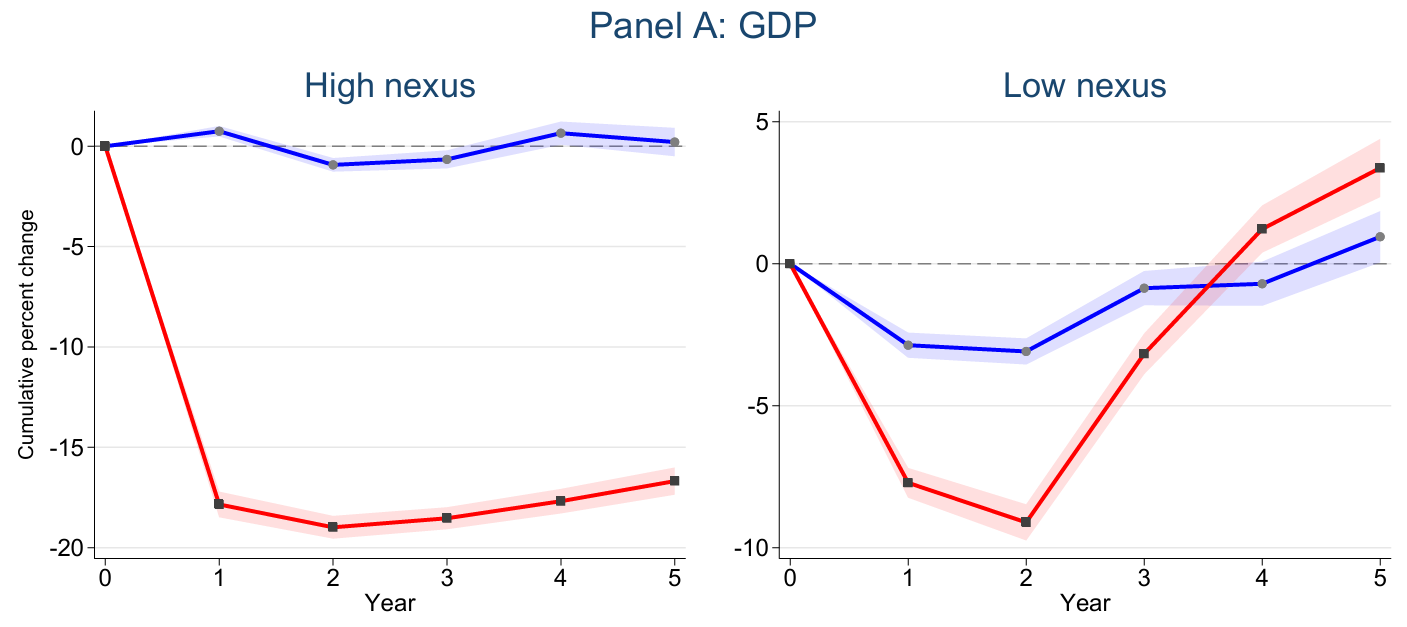
\includegraphics[width=0.95\textwidth]{figures/figB1_mean_precrisis.png}
\caption{Key variables around debt spread crises with pre-crisis periods, mean.}
\label{fig:B1}
\end{figure}

\begin{figure}[htbp]
\centering
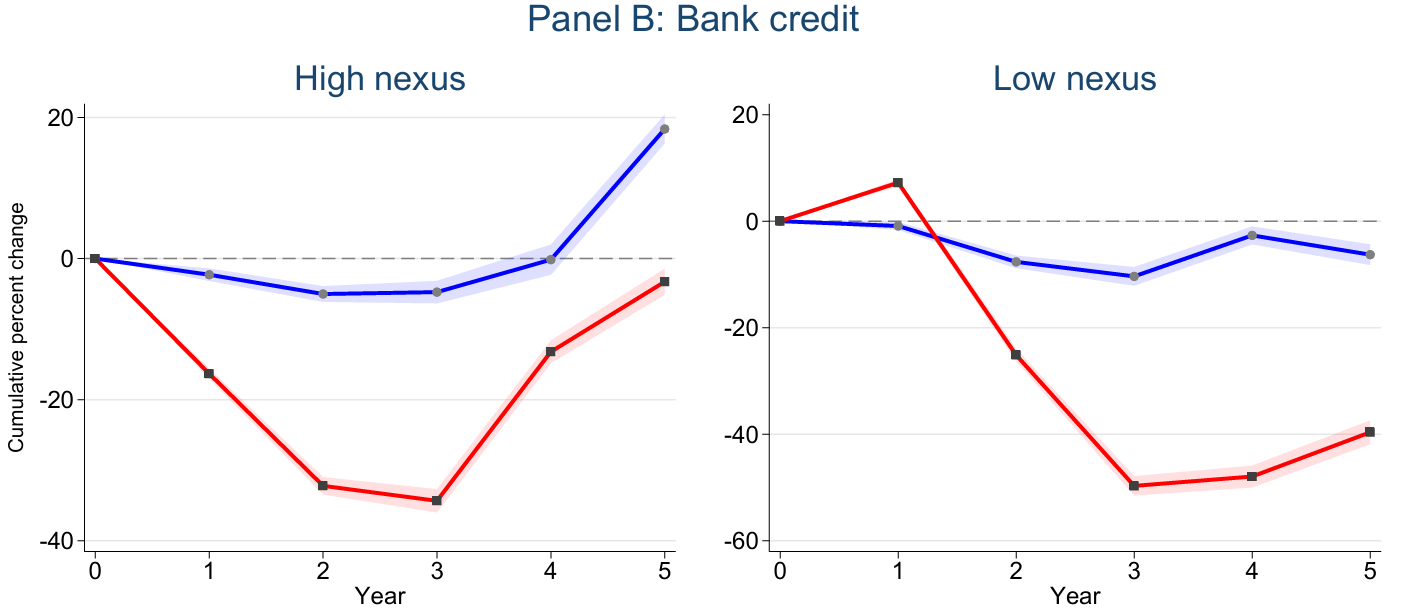
\includegraphics[width=0.95\textwidth]{figures/figB2_median_dynamics.png}
\caption{Key variables around debt spread crises, median.}
\label{fig:B2}
\end{figure}

\begin{figure}[htbp]
\centering
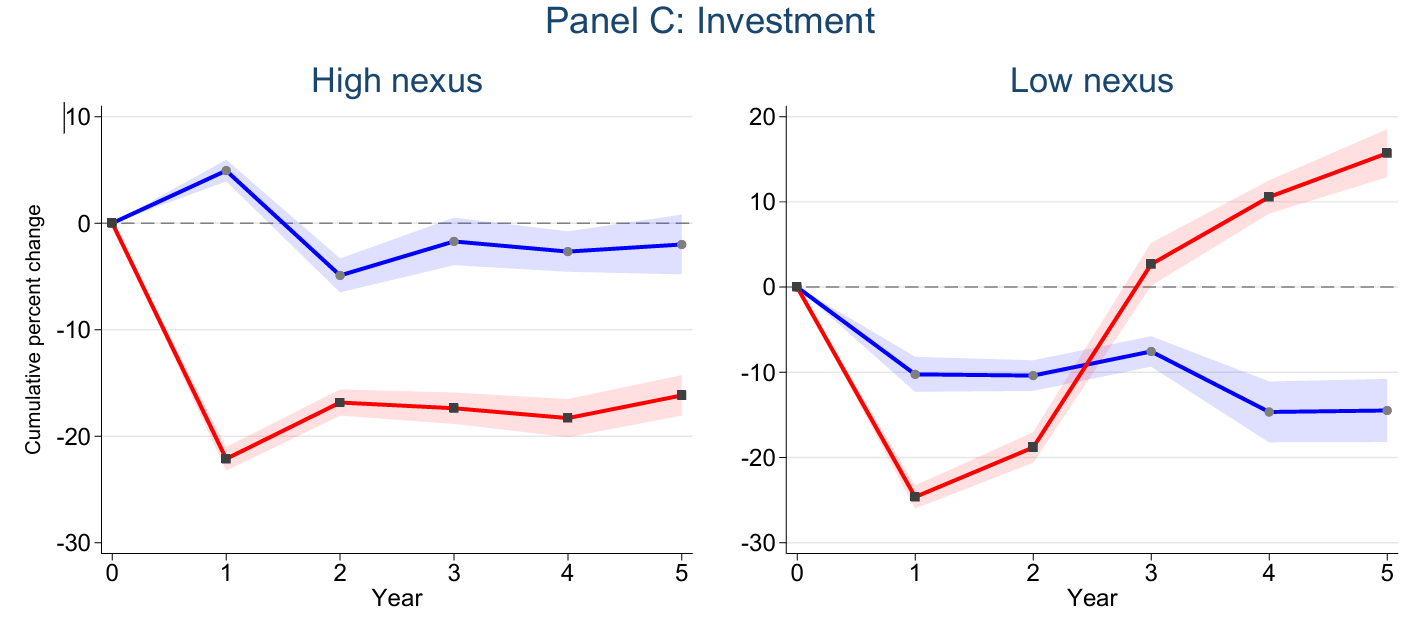
\includegraphics[width=0.95\textwidth]{figures/figB3_median_precrisis.png}
\caption{Key variables around debt spread crises with pre-crisis periods, median.}
\label{fig:B3}
\end{figure}

\begin{figure}[htbp]
\centering
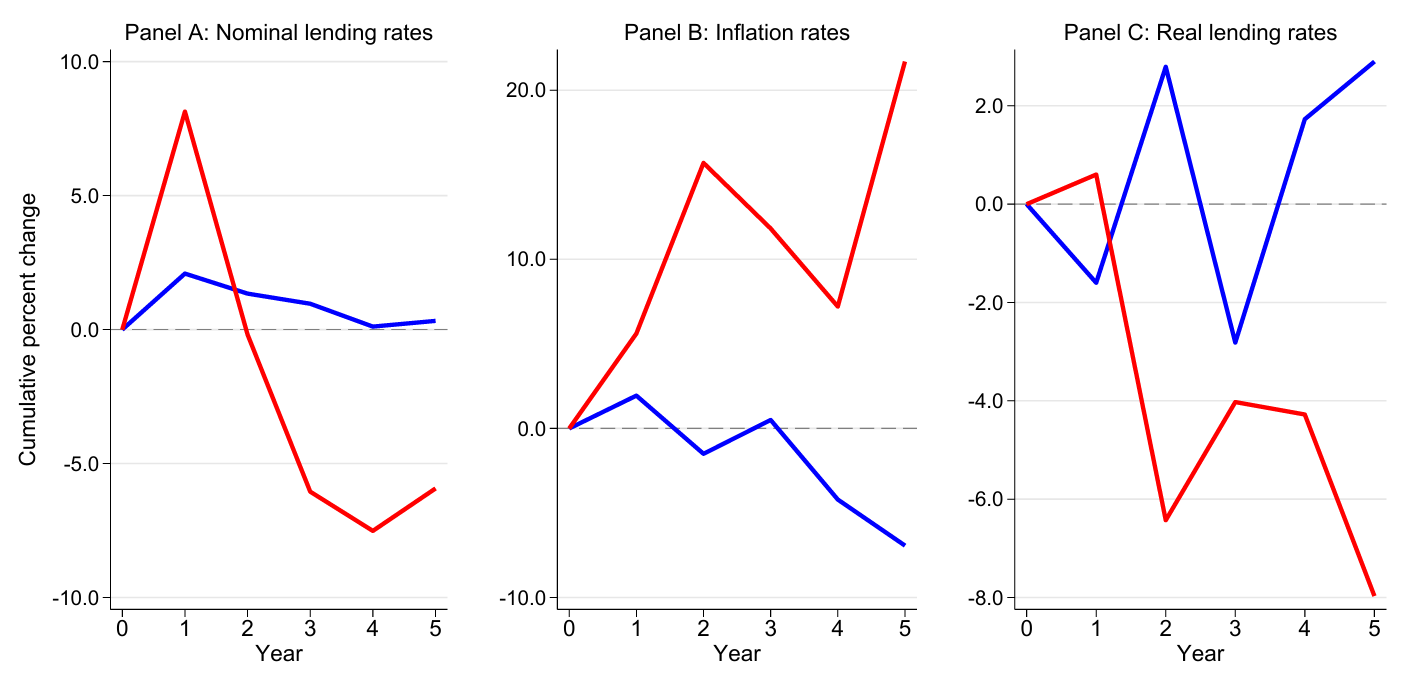
\includegraphics[width=0.95\textwidth]{figures/figB4_extra_macro.png}
\caption{Additional macroeconomic variables around spread crisis, mean.}
\label{fig:B4}
\end{figure}

% ============================================================
\section{Baseline OLS Regression}
% ============================================================

\begin{table}[p]
\centering
\caption{Estimation results, OLS}
\label{tab:C1}
\footnotesize
\begin{tabular}{lccccc}
\toprule
\multicolumn{6}{l}{\textbf{Panel A: GDP}} \\
 & $h=1$ & $h=2$ & $h=3$ & $h=4$ & $h=5$ \\
\midrule
Non-default & $-$0.82 & $-$2.79** & $-$0.60 & 0.69 & 0.61 \\
 & (1.17) & (1.13) & (1.07) & (1.37) & (1.42) \\
Obs./Countries/Episodes & 640/26/32 & 640/26/32 & 640/25/31 & 640/25/31 & 640/24/30 \\
Default-linked & $-$5.87*** & $-$8.70*** & $-$5.36** & $-$3.77 & $-$4.86 \\
 & (1.20) & (2.28) & (2.48) & (3.03) & (3.97) \\
Obs./Countries/Episodes & 631/10/16 & 631/10/16 & 631/10/16 & 631/10/16 & 631/10/16 \\
Difference [bootstrap 95\% CI] & [$-$8.34,$-$1.74]* & [$-$10.72,$-$0.74]* & [$-$9.89,0.58] & [$-$11.21,2.01] & [$-$14.44,3.98] \\
(Clogg $z$) & ($-$3.02***) & ($-$2.32**) & ($-$1.77*) & ($-$1.34) & ($-$1.30) \\
\addlinespace
\multicolumn{6}{l}{\textbf{Panel B: Bank credit}} \\
 & $h=1$ & $h=2$ & $h=3$ & $h=4$ & $h=5$ \\
\midrule
Non-default & $-$2.58 & $-$5.79* & $-$5.01* & $-$1.77 & $-$1.34 \\
 & (2.04) & (3.06) & (2.76) & (3.94) & (4.83) \\
Obs./Countries/Episodes & 627/20/25 & 627/19/24 & 627/18/23 & 627/17/22 & 627/16/20 \\
Default-linked & $-$2.69 & $-$20.67*** & $-$27.96** & $-$29.30** & $-$26.50** \\
 & (3.36) & (7.45) & (11.49) & (11.77) & (11.45) \\
Obs./Countries/Episodes & 619/8/12 & 619/8/12 & 619/8/12 & 619/8/11 & 619/8/11 \\
Difference [bootstrap 95\% CI] & [$-$8.65,7.54] & [$-$29.23,$-$0.32]* & [$-$45.41,$-$2.75]* & [$-$49.34,$-$5.98]* & [$-$47.62,$-$0.35]* \\
(Clogg $z$) & ($-$0.03) & ($-$1.85*) & ($-$1.94*) & ($-$2.22**) & ($-$2.02**) \\
\addlinespace
\multicolumn{6}{l}{\textbf{Panel C: Investment}} \\
 & $h=1$ & $h=2$ & $h=3$ & $h=4$ & $h=5$ \\
\midrule
Non-default & $-$1.14 & $-$12.86*** & $-$6.25 & $-$10.55* & $-$5.20 \\
 & (4.90) & (3.49) & (4.14) & (6.29) & (6.81) \\
Obs./Countries/Episodes & 640/25/31 & 640/25/31 & 640/24/30 & 640/24/30 & 640/23/29 \\
Default-linked & $-$4.89 & $-$20.04*** & $-$12.19 & $-$11.62 & $-$11.67 \\
 & (3.82) & (5.86) & (10.71) & (12.67) & (13.67) \\
Obs./Countries/Episodes & 631/10/16 & 631/10/16 & 631/10/16 & 631/10/16 & 631/10/16 \\
Difference [bootstrap 95\% CI] & [$-$17.45,10.13] & [$-$23.45,9.81] & [$-$28.70,16.86] & [$-$30.11,26.27] & [$-$37.15,25.88] \\
(Clogg $z$) & ($-$0.60) & ($-$1.05) & ($-$0.52) & ($-$0.07) & ($-$0.42) \\
\bottomrule
\end{tabular}
\end{table}

\begin{table}[p]
\centering
\ContinuedFloat
\footnotesize
\begin{tabular}{lccccc}
\toprule
\multicolumn{6}{l}{\textbf{Panel D: Bank claims on government}} \\
 & $h=1$ & $h=2$ & $h=3$ & $h=4$ & $h=5$ \\
\midrule
Non-default & 0.36 & 0.61 & 0.57 & $-$0.20 & 0.64 \\
 & (0.88) & (1.08) & (1.21) & (1.39) & (1.93) \\
Obs./Countries/Episodes & 639/26/31 & 639/25/30 & 639/24/29 & 639/23/28 & 639/22/26 \\
Default-linked & 4.46** & 5.15 & 4.18 & 0.44 & $-$0.70 \\
 & (1.88) & (3.83) & (2.90) & (1.64) & (1.60) \\
Obs./Countries/Episodes & 630/9/15 & 630/9/15 & 630/9/15 & 630/9/15 & 630/9/14 \\
Difference [bootstrap 95\% CI] & [0.55,7.72]* & [$-$1.48,11.45] & [$-$2.38,9.07] & [$-$4.05,4.90] & [$-$6.96,4.34] \\
(Clogg $z$) & (1.98**) & (1.14) & (1.15) & (0.29) & ($-$0.54) \\
\addlinespace
\multicolumn{6}{l}{\textbf{Panel E: FDI}} \\
 & $h=1$ & $h=2$ & $h=3$ & $h=4$ & $h=5$ \\
\midrule
Non-default & $-$0.39 & $-$0.45 & $-$0.66 & $-$0.31 & 0.07 \\
 & (0.51) & (0.78) & (0.85) & (0.87) & (0.84) \\
Obs./Countries/Episodes & 893/24/30 & 857/24/30 & 822/24/30 & 788/22/28 & 750/21/25 \\
Default-linked & $-$0.75 & $-$0.71 & $-$0.11 & $-$0.28 & 0.59 \\
 & (0.60) & (0.59) & (0.54) & (0.73) & (0.94) \\
Obs./Countries/Episodes & 879/10/16 & 843/10/16 & 808/10/16 & 775/10/15 & 740/10/15 \\
Difference [bootstrap 95\% CI] & [$-$2.38,1.33] & [$-$2.68,1.86] & [$-$1.81,3.45] & [$-$2.61,2.77] & [$-$2.62,3.59] \\
(Clogg $z$) & ($-$0.47) & ($-$0.27) & (0.55) & (0.03) & (0.42) \\
\addlinespace
\multicolumn{6}{l}{\textbf{Panel F: Real lending rate}} \\
 & $h=1$ & $h=2$ & $h=3$ & $h=4$ & $h=5$ \\
\midrule
Non-default & $-$1.66* & 2.51 & $-$2.78 & 0.62 & 2.36 \\
 & (0.92) & (1.67) & (3.22) & (2.33) & (1.96) \\
Obs./Countries/Episodes & 658/18/19 & 626/18/19 & 594/18/19 & 558/14/14 & 523/14/14 \\
Default-linked & $-$0.44 & $-$7.48* & $-$1.30 & $-$3.88 & $-$7.16 \\
 & (6.27) & (4.26) & (3.61) & (2.42) & (4.47) \\
Obs./Countries/Episodes & 649/6/10 & 617/6/10 & 584/5/9 & 553/5/9 & 517/5/8 \\
Difference [bootstrap 95\% CI] & [$-$9.58,13.56] & [$-$19.14,0.89] & [$-$8.03,11.28] & [$-$13.48,5.30] & [$-$18.75,$-$0.11]* \\
(Clogg $z$) & (0.19) & ($-$2.18**) & (0.31) & ($-$1.34) & ($-$1.95*) \\
\bottomrule
\end{tabular}
\notes{Estimates are from OLS, rather than AIPW, local projections;
otherwise the specification, sample, and testing conventions match
Table~2. * p$<$0.10, ** p$<$0.05, *** p$<$0.01.}
\end{table}

\clearpage

% ============================================================
\section{Treatment and Control Groups, and First-Stage Results}
% ============================================================

\begin{table}[htbp]
\centering
\caption{Regression of each type of spread crisis on control variables}
\label{tab:D1}
\footnotesize
\begin{tabular}{lcccccccc}
\toprule
 & GDP growth & Debt/GDP & Bank crisis & Govt.\ exp./GDP & Openness & Credit/GDP & Log infl.\ & Exch.\ rate \\
\midrule
Non-default & 0.88 & 1.03 & 0.08 & $-$1.71 & $-$10.88* & $-$9.30** & 0.02 & 0.00 \\
 & (0.54) & (5.69) & (0.06) & (1.42) & (6.16) & (4.63) & (0.01) & (0.01) \\
Default-linked & $-$2.53*** & 10.89 & 0.09 & 0.25 & $-$7.44 & $-$9.86 & 0.18 & 0.06* \\
 & (0.90) & (7.00) & (0.08) & (2.11) & (5.83) & (6.57) & (0.14) & (0.03) \\
\addlinespace
Observations & 1085 & 1056 & 1085 & 1063 & 998 & 1069 & 1076 & 1081 \\
Countries & 51 & 51 & 51 & 51 & 47 & 51 & 51 & 51 \\
R-squared & 0.0118 & 0.0029 & 0.0071 & 0.0013 & 0.0039 & 0.0057 & 0.0473 & 0.0057 \\
\bottomrule
\end{tabular}
\notes{Each column is a separate regression of that control variable (at
$t-1$) on \texttt{onset\_nd} and \texttt{onset\_def} jointly, on the full
sample (tranquil years plus both onset types); tranquil years are the
omitted/reference category, so each coefficient shown is that arm's mean
difference from tranquil years. Robust standard errors in parentheses.
* p$<$0.10, ** p$<$0.05, *** p$<$0.01.}
\end{table}

\begin{figure}[htbp]
\centering
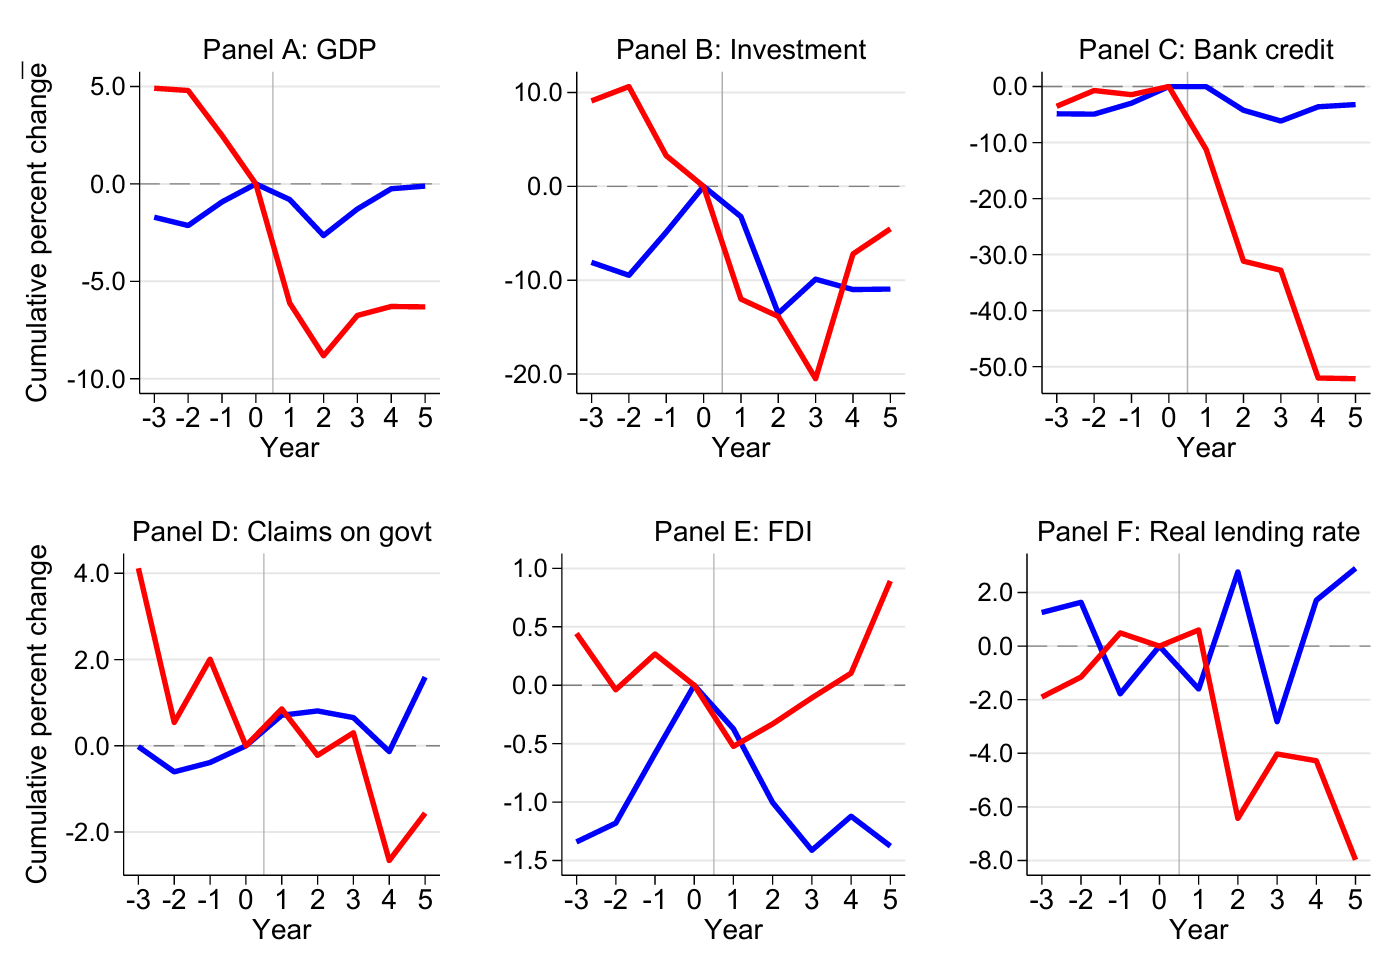
\includegraphics[width=0.8\textwidth]{figures/figD1_roc_curves.png}
\caption{Classification power of the probit regression regressors, ROC curves.}
\label{fig:D1}
\notes{Each panel shows the area under the ROC curve. The area under the
ROC ranges from 0.50 (predictors have no classification power when
differentiating the start of a spread crisis from other observations) to
1.00 (perfect classification power).}
\end{figure}

\end{document}
